\documentclass[a4j]{jarticle}
\usepackage[dvipdfmx]{graphicx}
\usepackage{amssymb}
\usepackage{subfigure}
\usepackage{longtable}

\begin{document}
\begin{table}[t]
\begin{center}
{\large 産業用モニタリングシステムにおける障害検知手法の提案}\\
令和 2 年 7 月 8 日\\
山本 航平
\end{center}
\end{table}

進捗報告
\begin{itemize}
\item 6 月 23 日(火)から 15 秒間隔での継続的な計測を行っています
\item 7 月 7 日(火)から 10 秒間隔での継続的な計測を開始しました
\item LTE の接続切れのプロセスを調べました
\item LTE コアネットワーク内のタイマーについて調べました
\end{itemize}

\section{突発的に発生する大きな応答遅延の単発性の検証}
ping による応答遅延の計測を 10 ミリ秒間隔で計 10 回行う操作を 5 秒毎に実行した.また,計測期間は計 1 時間とした.ping コマンドの実行時刻が早いものから順に $t = 1,2,\ldots$ とし,$t$ を横軸に,縦軸にはそれに対応する ping 応答遅延時間 [ms] をとった結果を図 \ref{data1-1} から図 \ref{data1-2} に示す.この図では,縦軸に垂直な黒線で ping の実行時刻に応じた組分けをしており,組内の ping の実行間隔は 10 ミリ秒,組間の先頭の ping の実行間隔が 5 秒となるようにしている.
\begin{figure}[tb]
\begin{center}
\subfigure[$0 \sim 1$ 分後]{
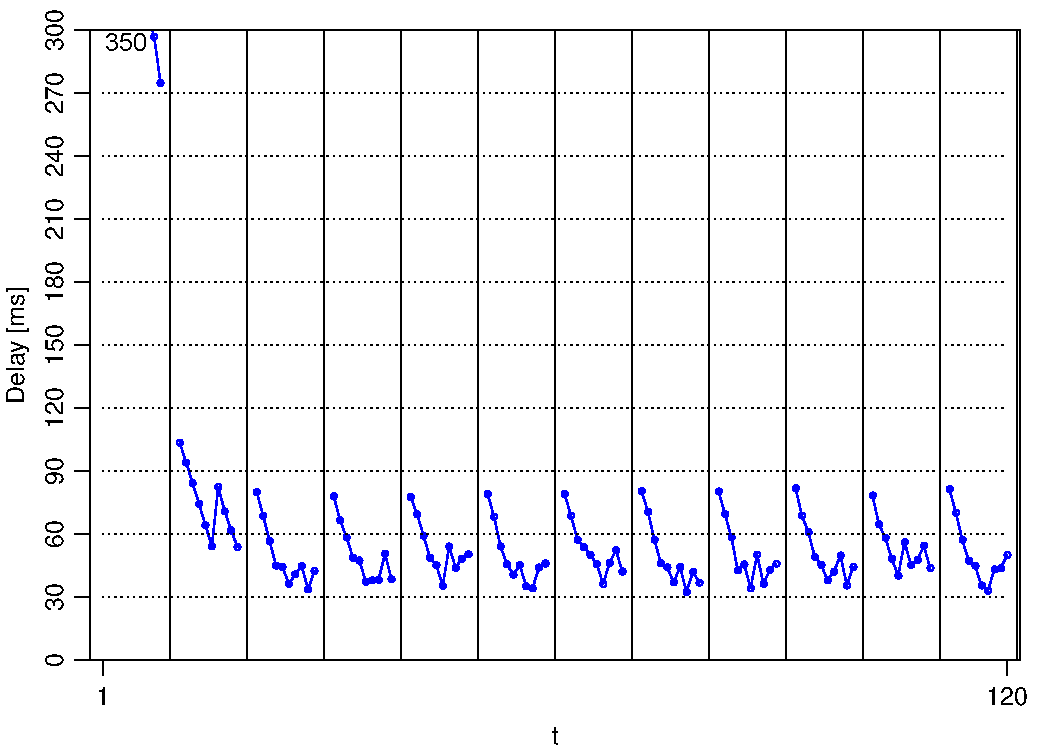
\includegraphics[width=0.33\hsize]{../2020-07-02/0-1.pdf}
}~
\subfigure[$1 \sim 2$ 分後]{
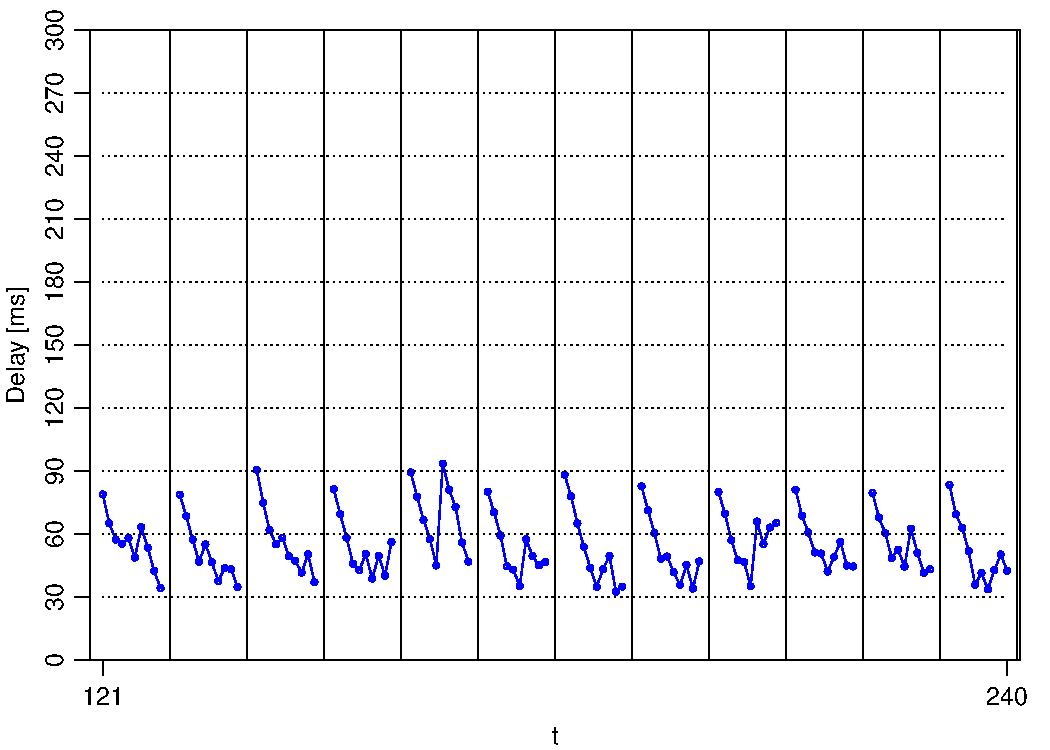
\includegraphics[width=0.33\hsize]{../2020-07-02/1-2.pdf}
}~
\subfigure[$2 \sim 3$ 分後]{
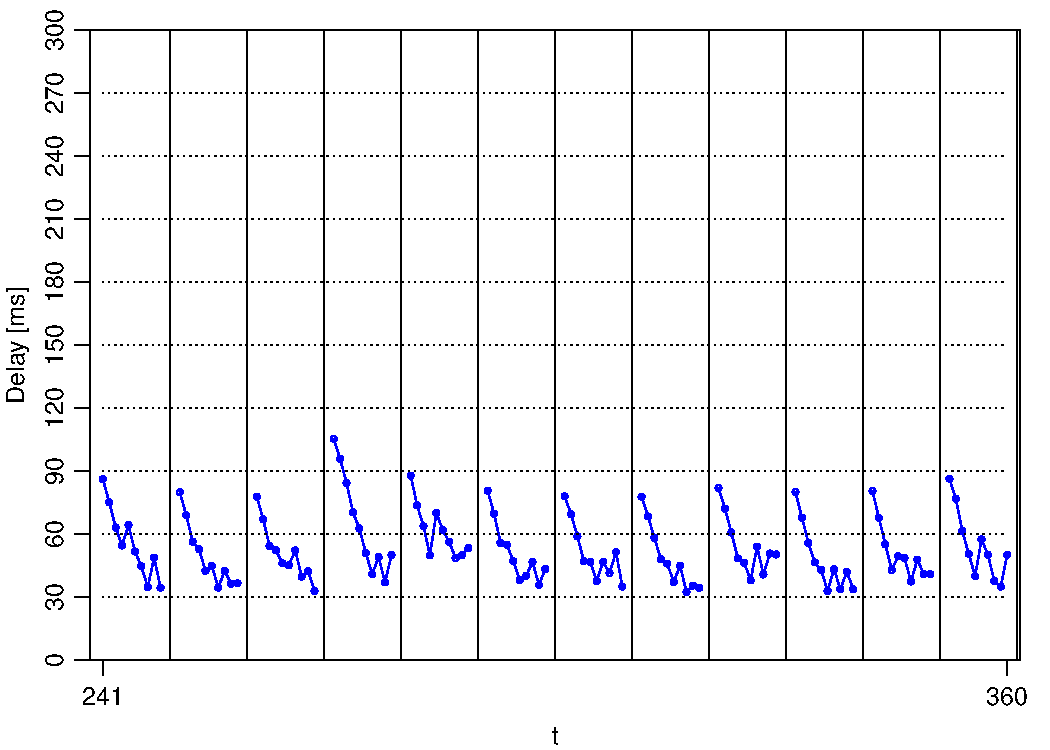
\includegraphics[width=0.33\hsize]{../2020-07-02/2-3.pdf}
}\\

\subfigure[$3 \sim 4$ 分後]{
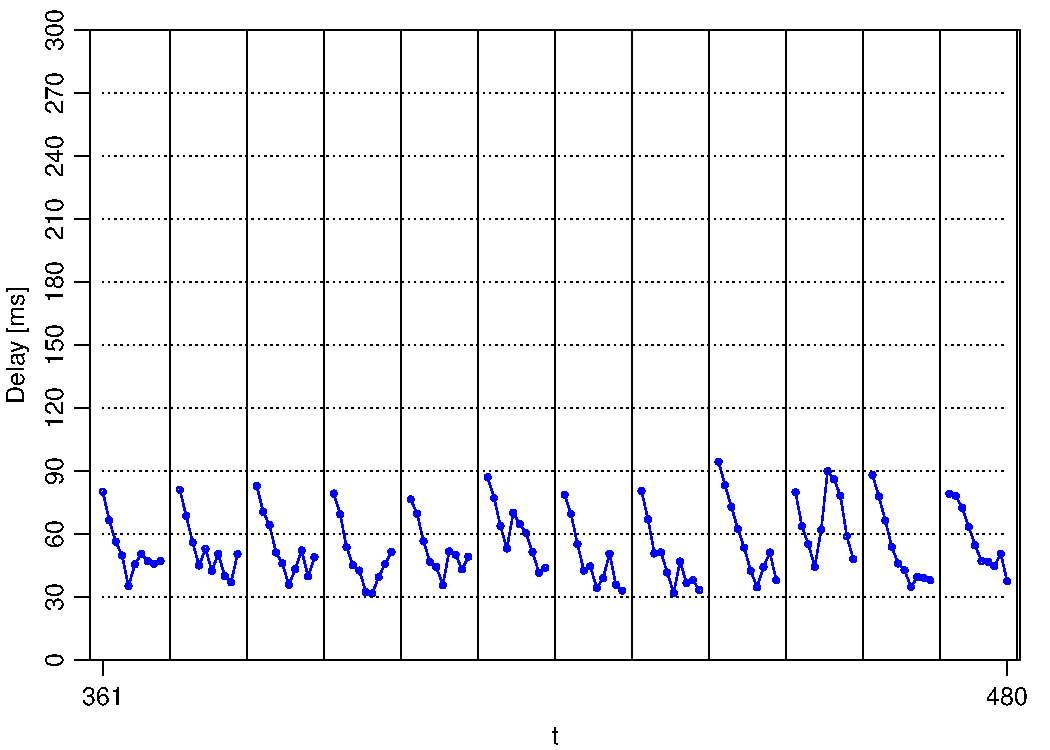
\includegraphics[width=0.33\hsize]{../2020-07-02/3-4.pdf}
}~
\subfigure[$4 \sim 5$ 分後]{
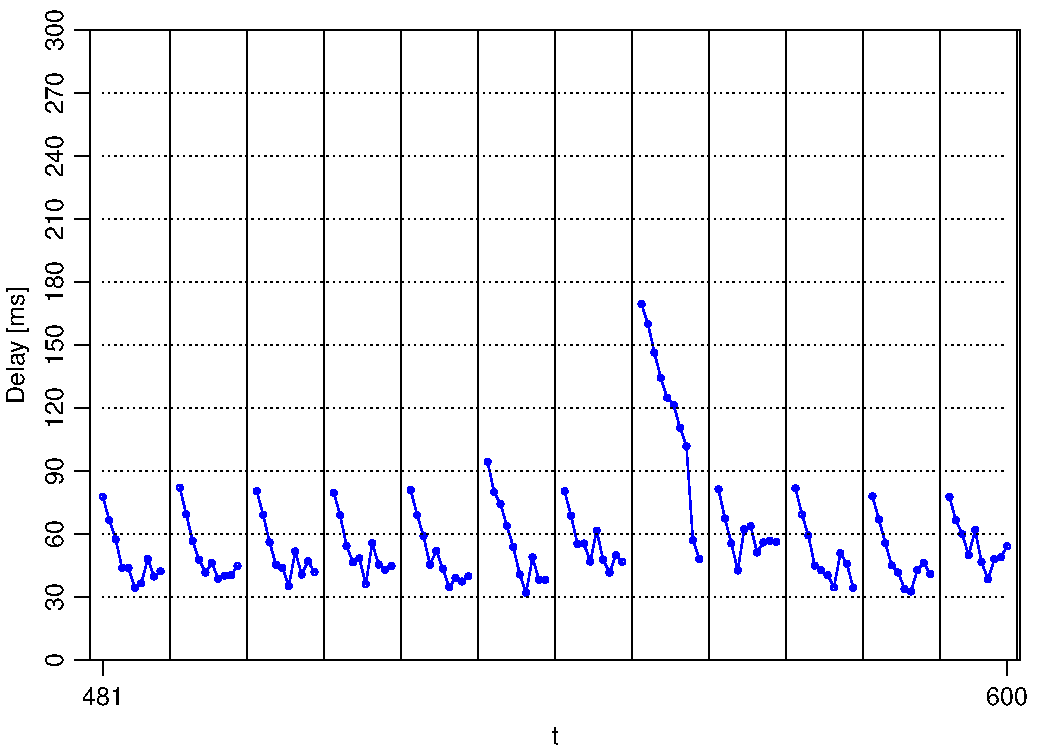
\includegraphics[width=0.33\hsize]{../2020-07-02/4-5.pdf}
}~
\subfigure[$5 \sim 6$ 分後]{
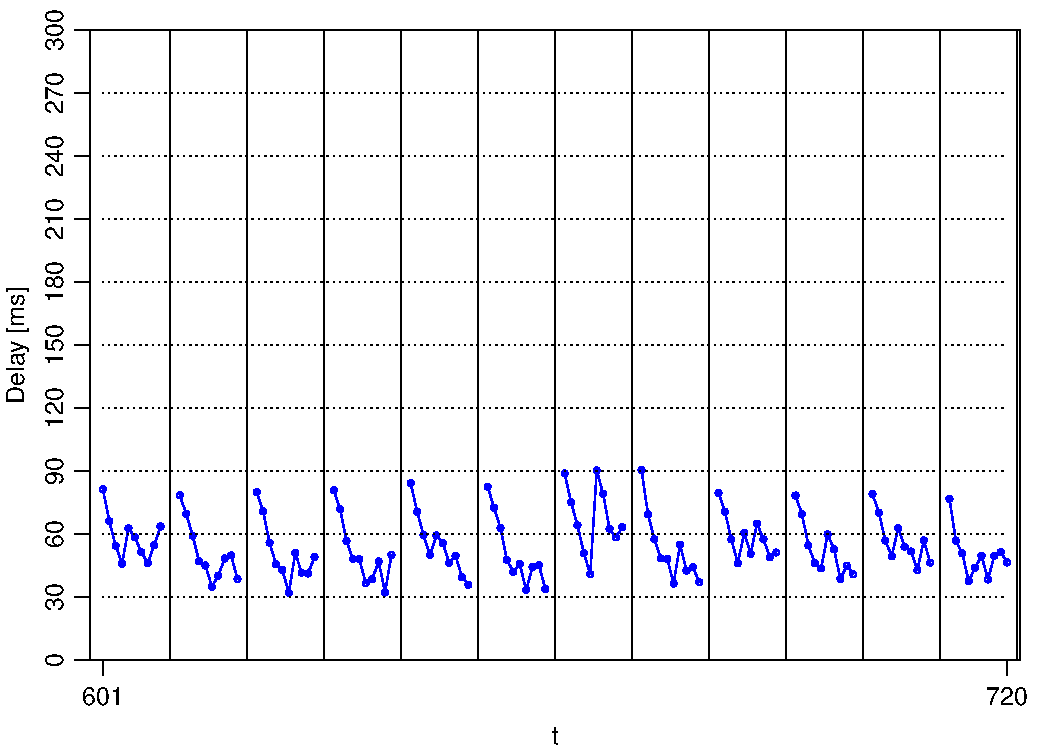
\includegraphics[width=0.33\hsize]{../2020-07-02/5-6.pdf}
}\\

\subfigure[$6 \sim 7$ 分後]{
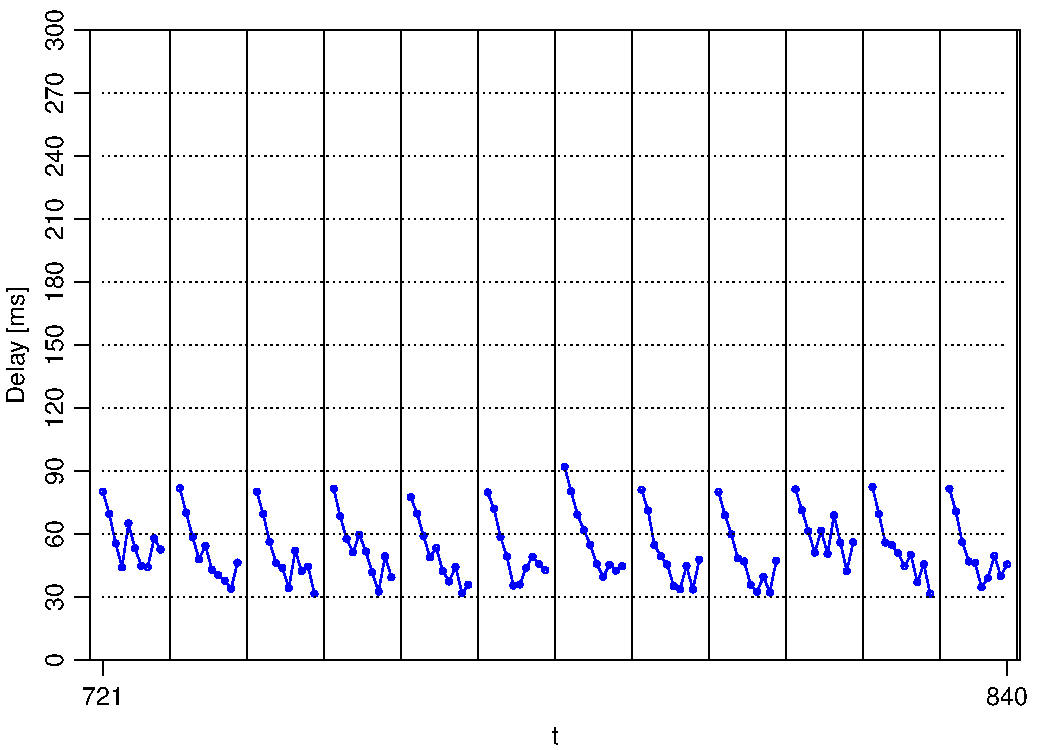
\includegraphics[width=0.33\hsize]{../2020-07-02/6-7.pdf}
}~
\subfigure[$7 \sim 8$ 分後]{
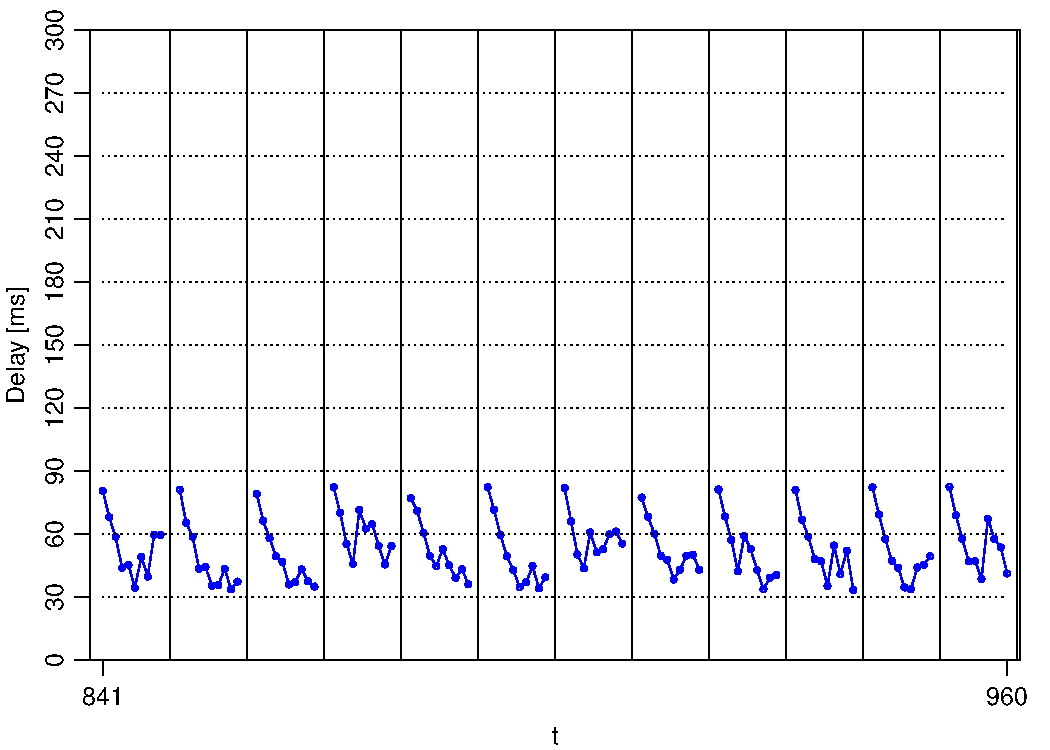
\includegraphics[width=0.33\hsize]{../2020-07-02/7-8.pdf}
}~
\subfigure[$8 \sim 9$ 分後]{
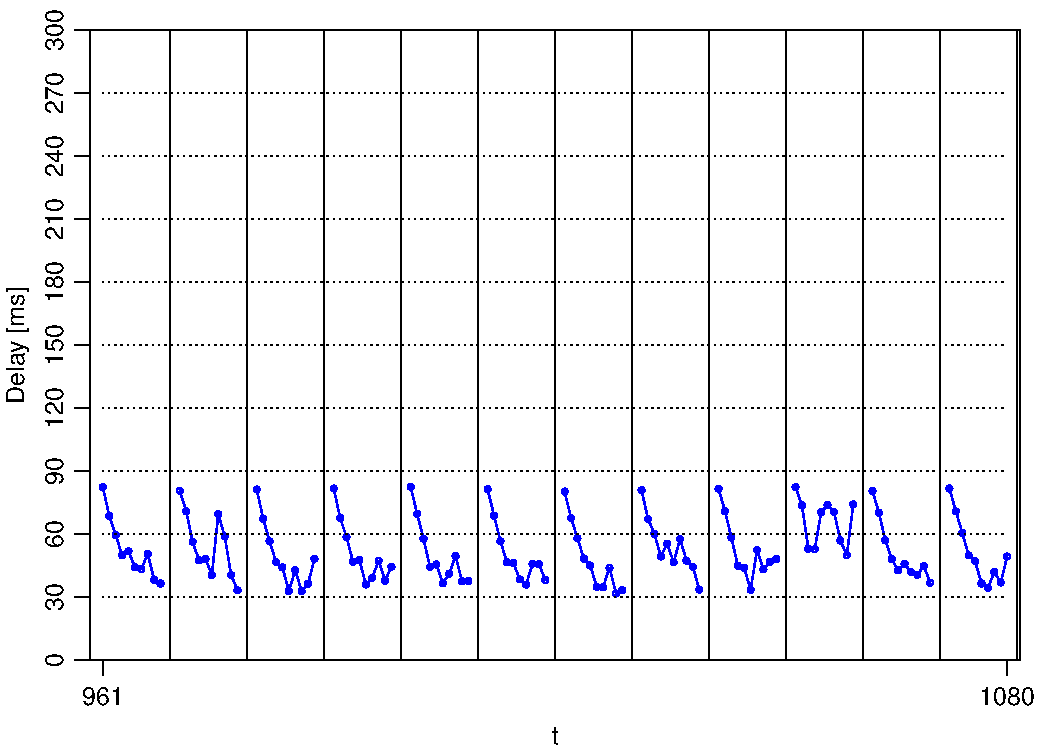
\includegraphics[width=0.33\hsize]{../2020-07-02/8-9.pdf}
}\\

\subfigure[$9 \sim 10$ 分後]{
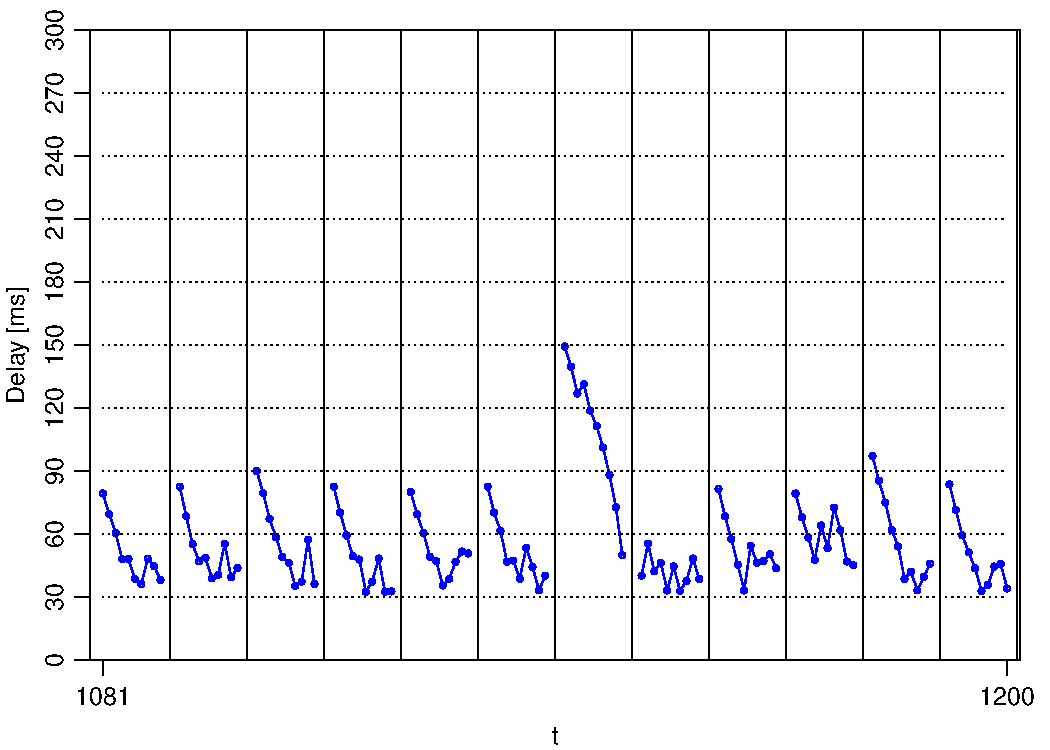
\includegraphics[width=0.33\hsize]{../2020-07-02/9-10.pdf}
}~
\subfigure[$10 \sim 11$ 分後]{
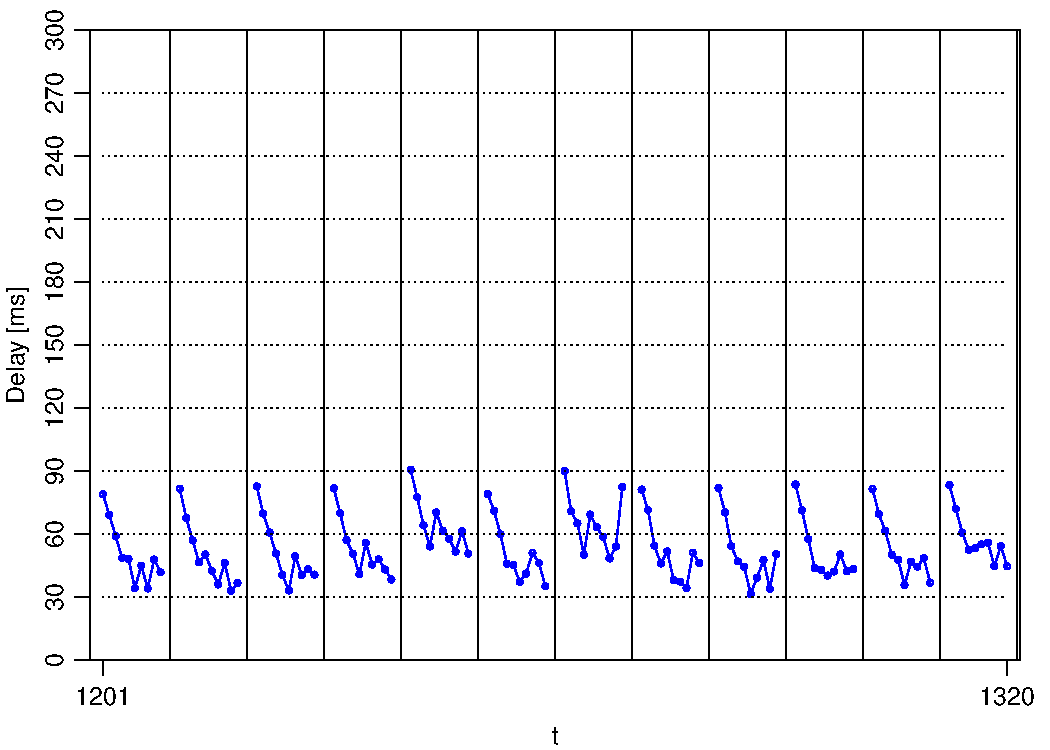
\includegraphics[width=0.33\hsize]{../2020-07-02/10-11.pdf}
}~
\subfigure[$11 \sim 12$ 分後]{
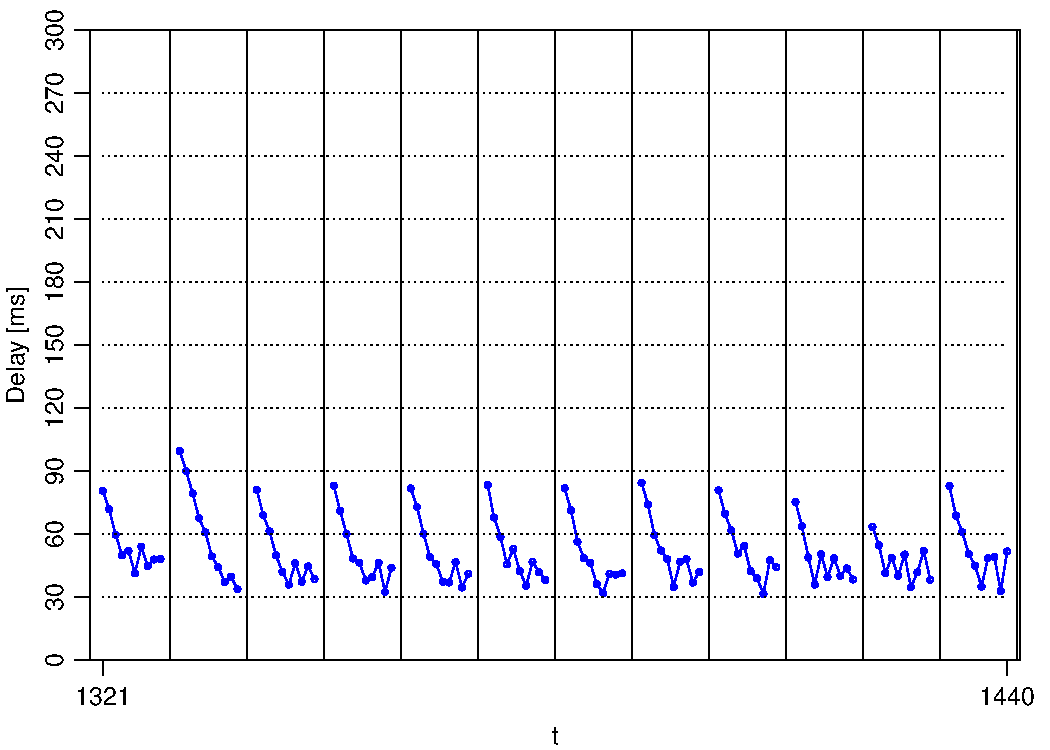
\includegraphics[width=0.33\hsize]{../2020-07-02/11-12.pdf}
}\\

\subfigure[$12 \sim 13$ 分後]{
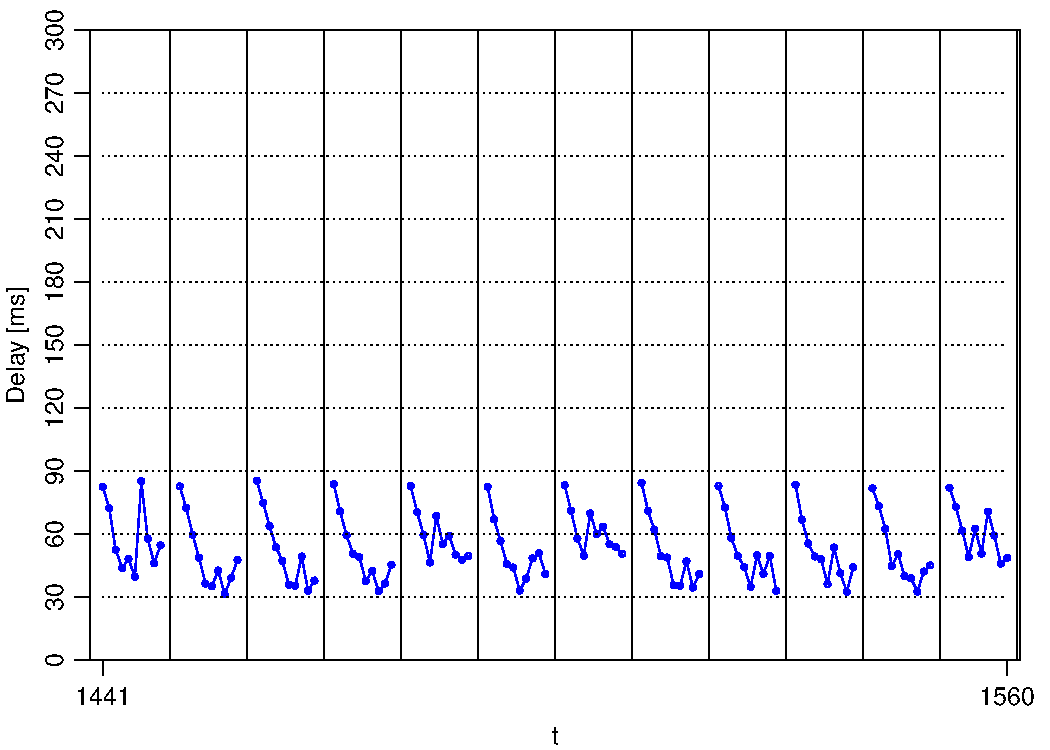
\includegraphics[width=0.33\hsize]{../2020-07-02/12-13.pdf}
}~
\subfigure[$13 \sim 14$ 分後]{
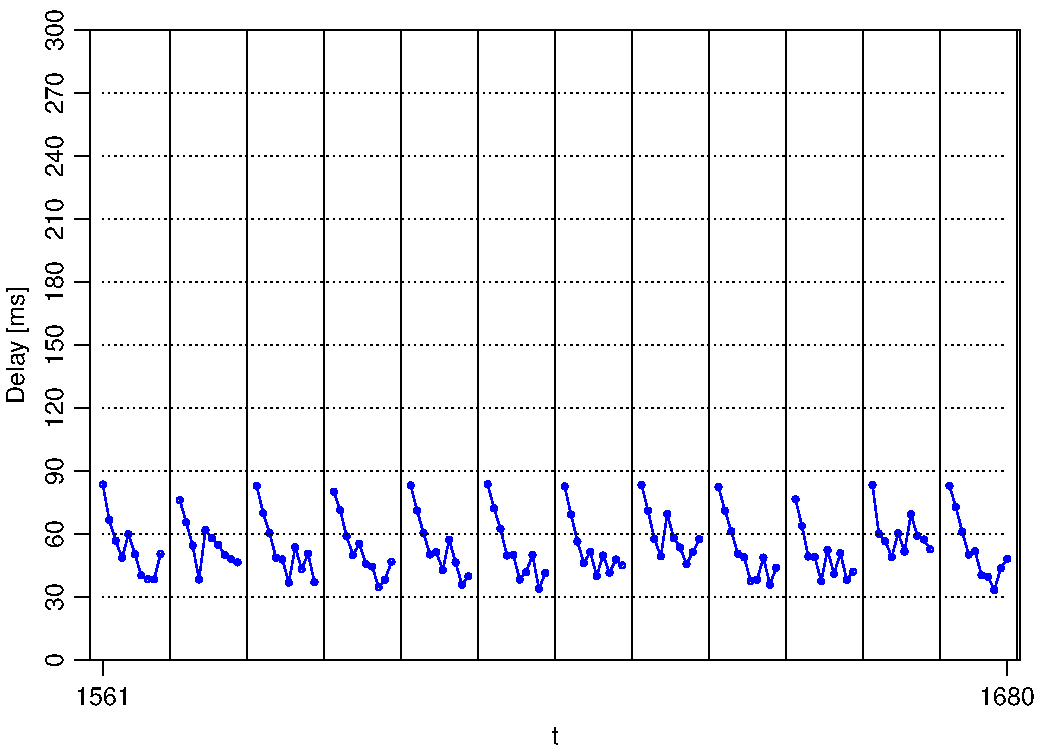
\includegraphics[width=0.33\hsize]{../2020-07-02/13-14.pdf}
}~
\subfigure[$14 \sim 15$ 分後]{
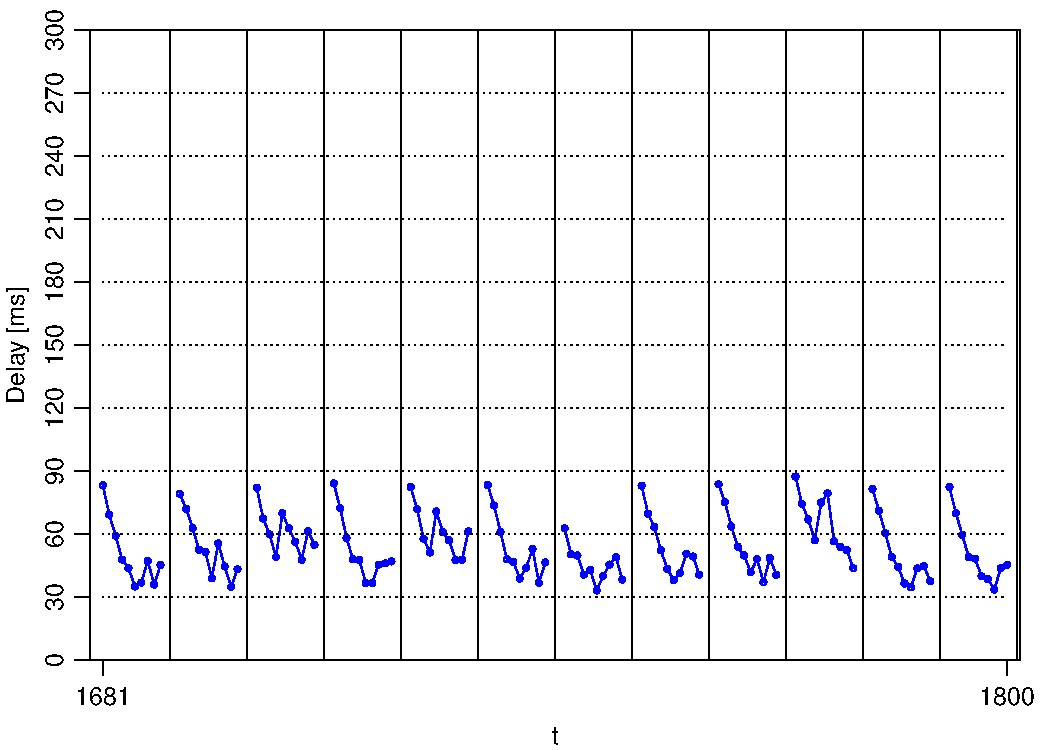
\includegraphics[width=0.33\hsize]{../2020-07-02/14-15.pdf}
}
\caption{10 ミリ秒間隔で計 10 回の ping 実行を 5 秒毎に行った計測結果(開始から 15 分後まで)}
\label{data1-1}
\end{center}
\end{figure}

\begin{figure}[tb]
\begin{center}
\subfigure[$15 \sim 16$ 分後]{
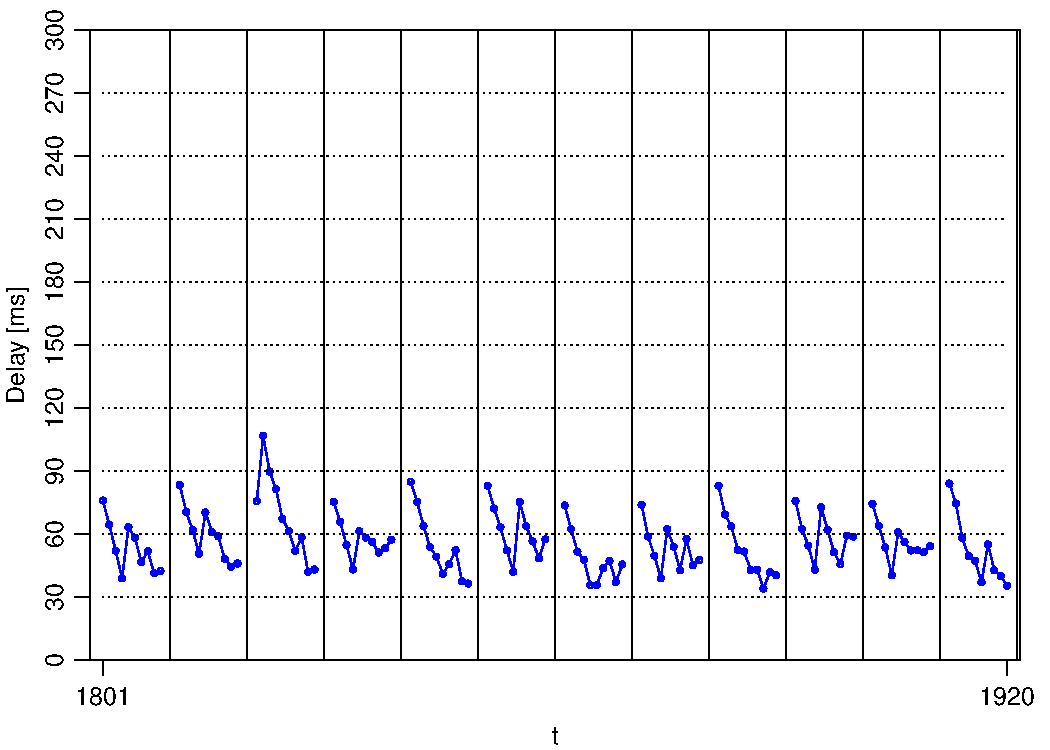
\includegraphics[width=0.33\hsize]{../2020-07-02/15-16.pdf}
}~
\subfigure[$16 \sim 17$ 分後]{
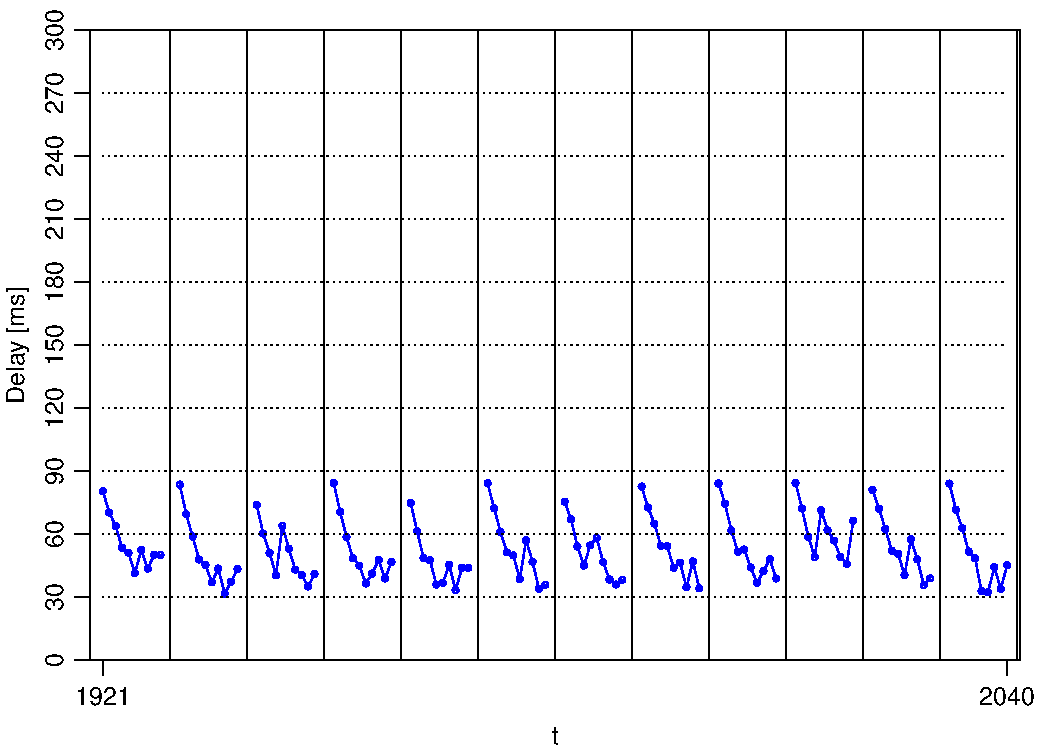
\includegraphics[width=0.33\hsize]{../2020-07-02/16-17.pdf}
}~
\subfigure[$17 \sim 18$ 分後]{
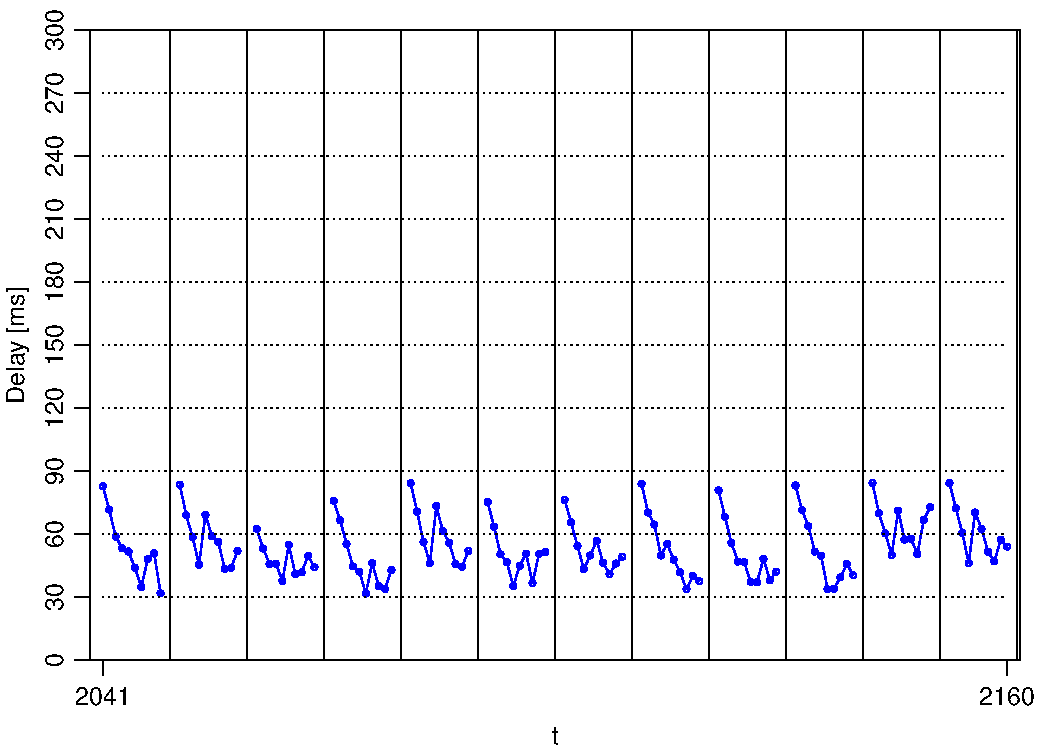
\includegraphics[width=0.33\hsize]{../2020-07-02/17-18.pdf}
}\\

\subfigure[$18 \sim 19$ 分後]{
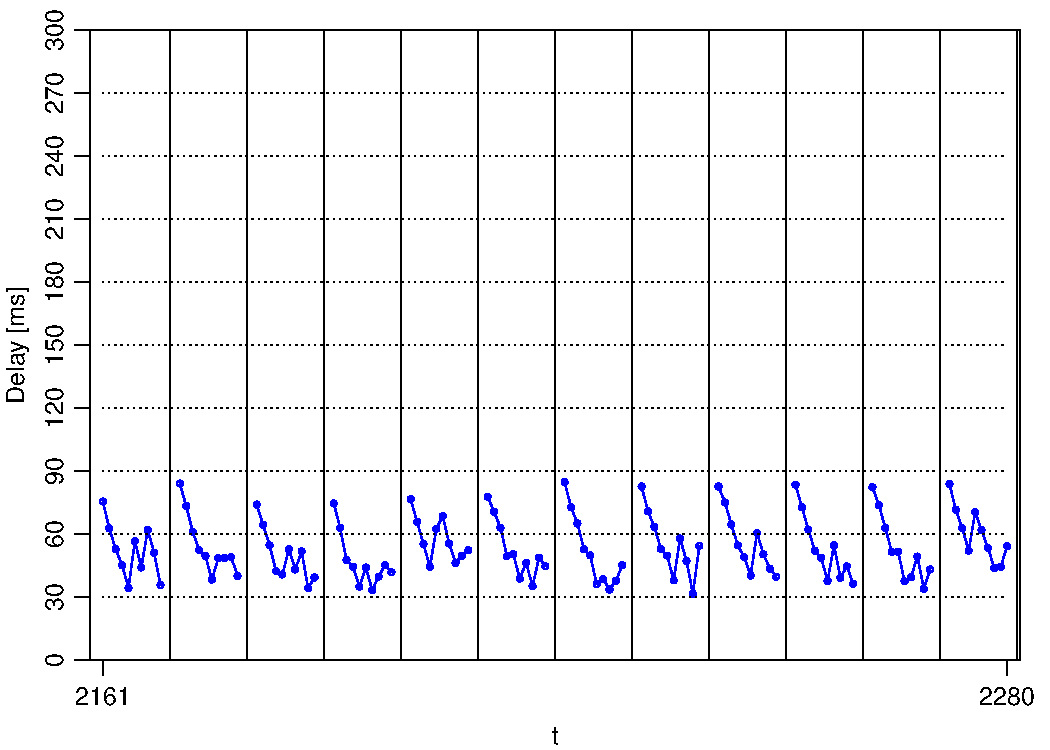
\includegraphics[width=0.33\hsize]{../2020-07-02/18-19.pdf}
}~
\subfigure[$19 \sim 20$ 分後]{
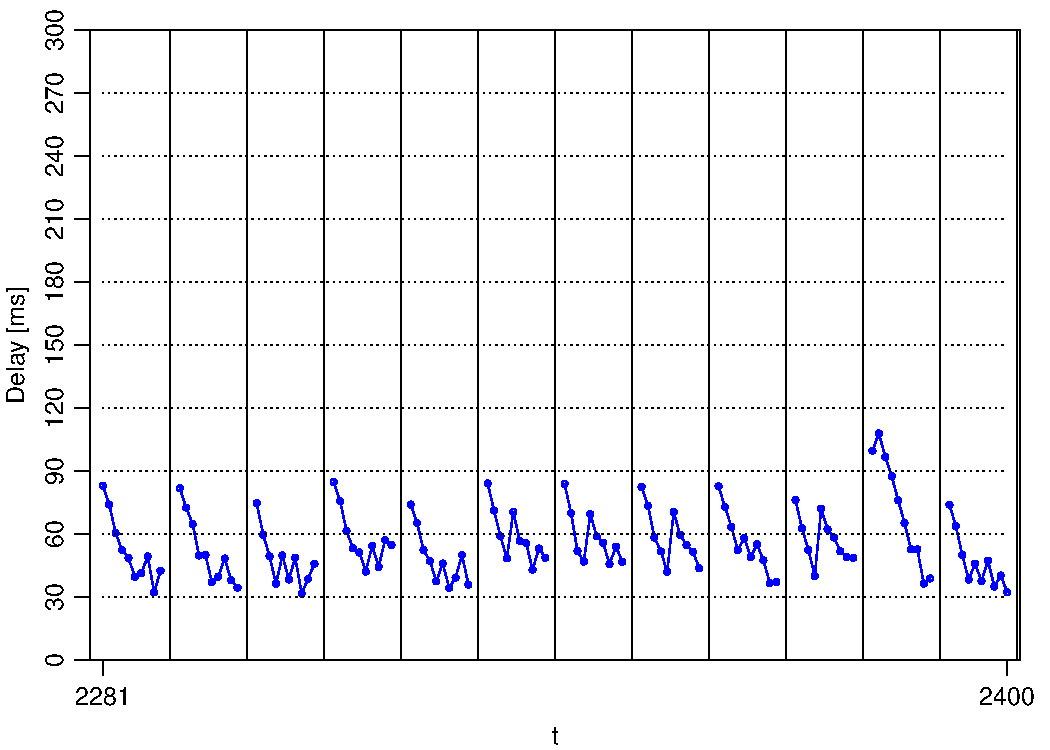
\includegraphics[width=0.33\hsize]{../2020-07-02/19-20.pdf}
}~
\subfigure[$20 \sim 21$ 分後]{
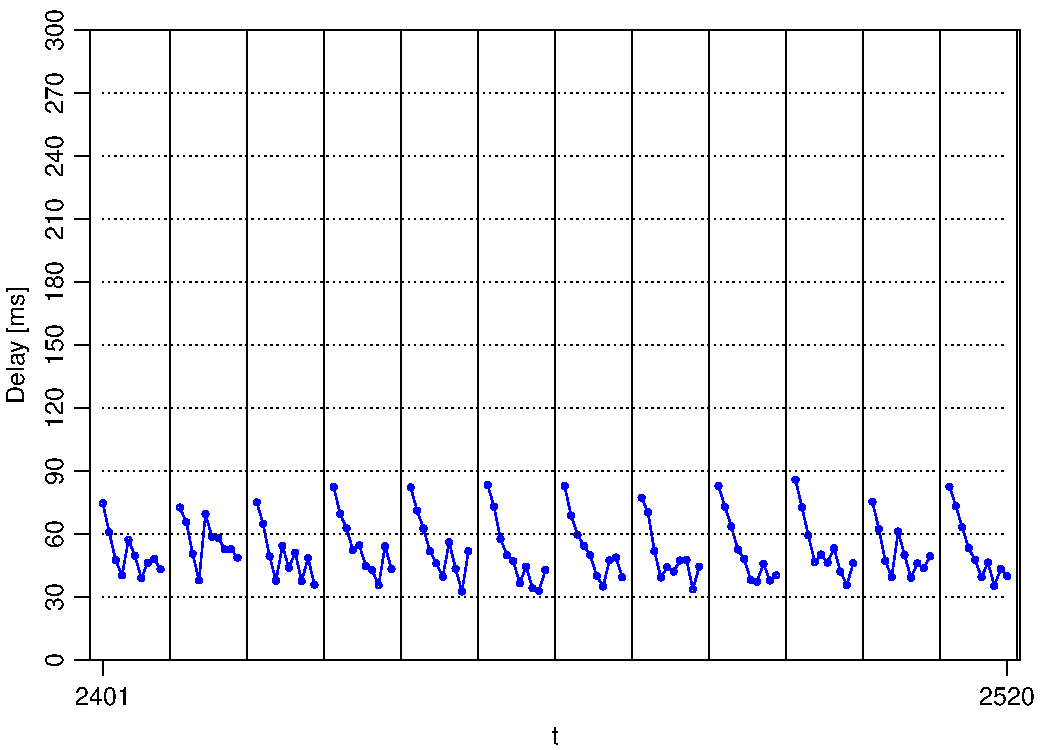
\includegraphics[width=0.33\hsize]{../2020-07-02/20-21.pdf}
}\\

\subfigure[$21 \sim 22$ 分後]{
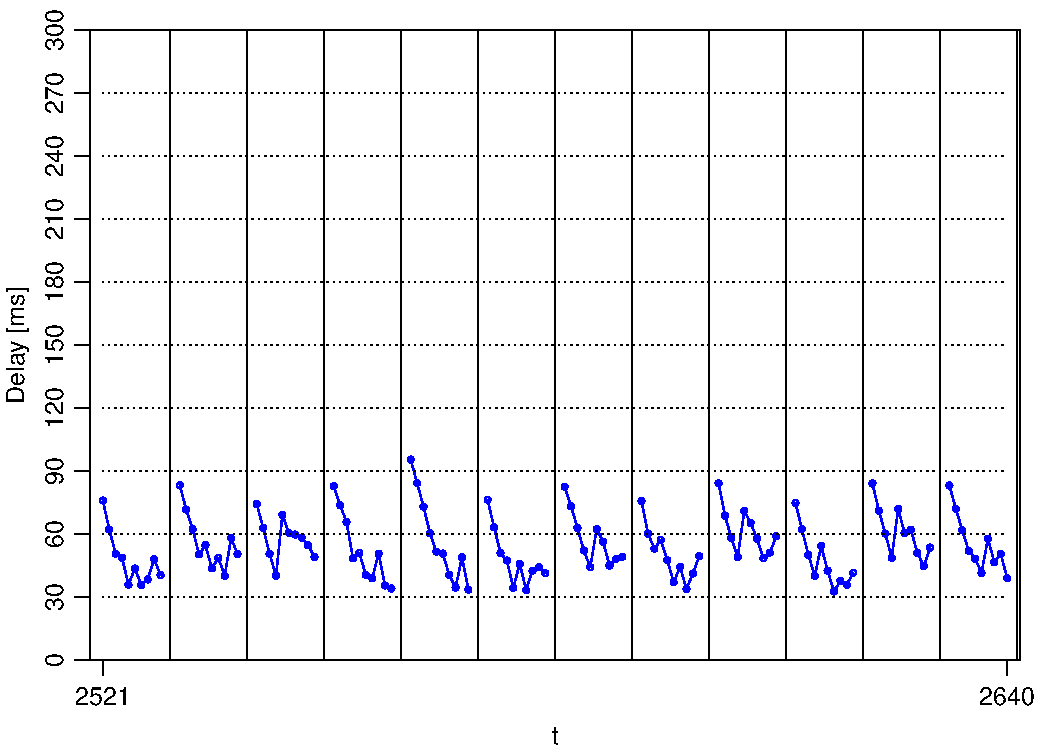
\includegraphics[width=0.33\hsize]{../2020-07-02/21-22.pdf}
}~
\subfigure[$22 \sim 23$ 分後]{
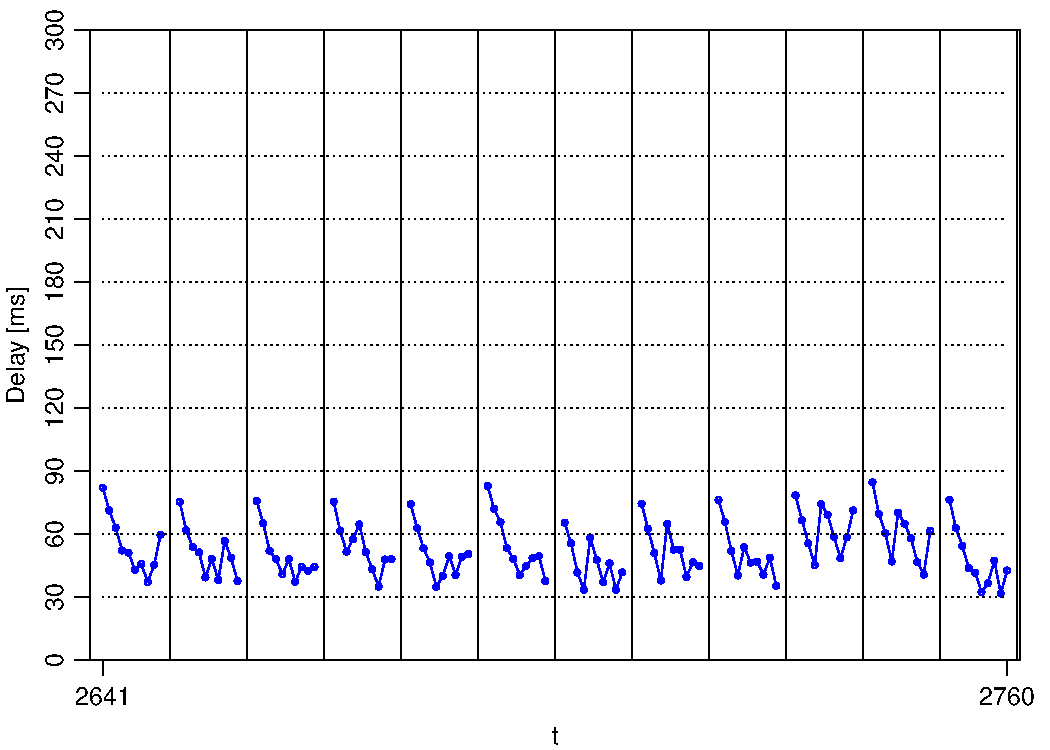
\includegraphics[width=0.33\hsize]{../2020-07-02/22-23.pdf}
}~
\subfigure[$23 \sim 24$ 分後]{
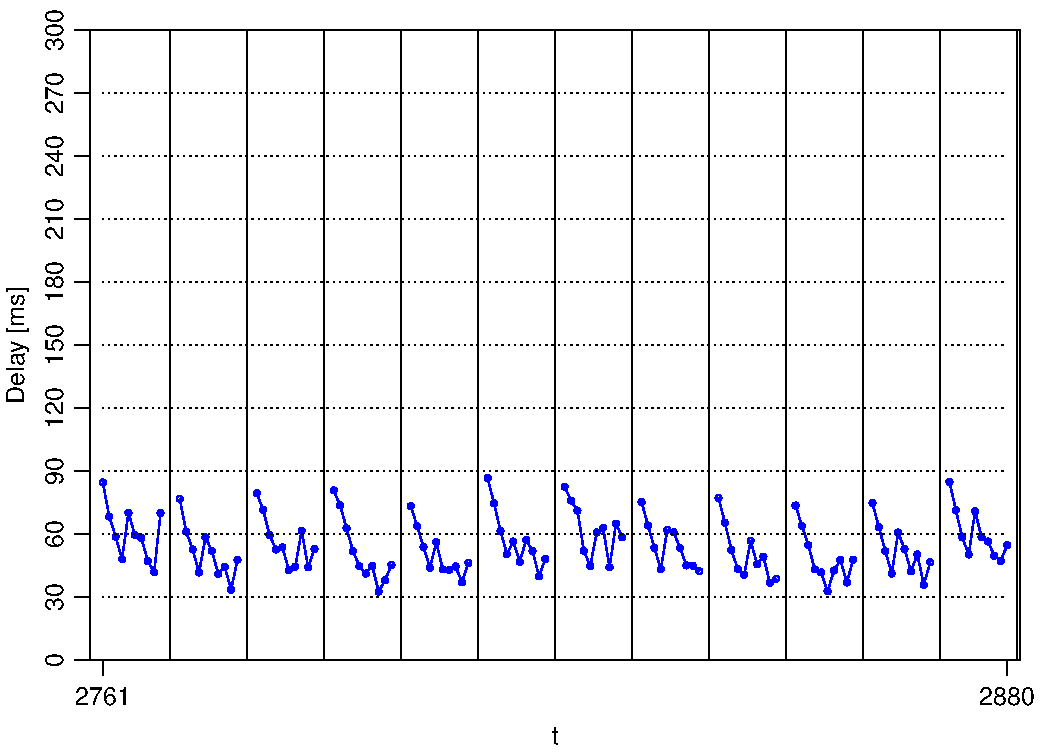
\includegraphics[width=0.33\hsize]{../2020-07-02/23-24.pdf}
}\\

\subfigure[$24 \sim 25$ 分後]{
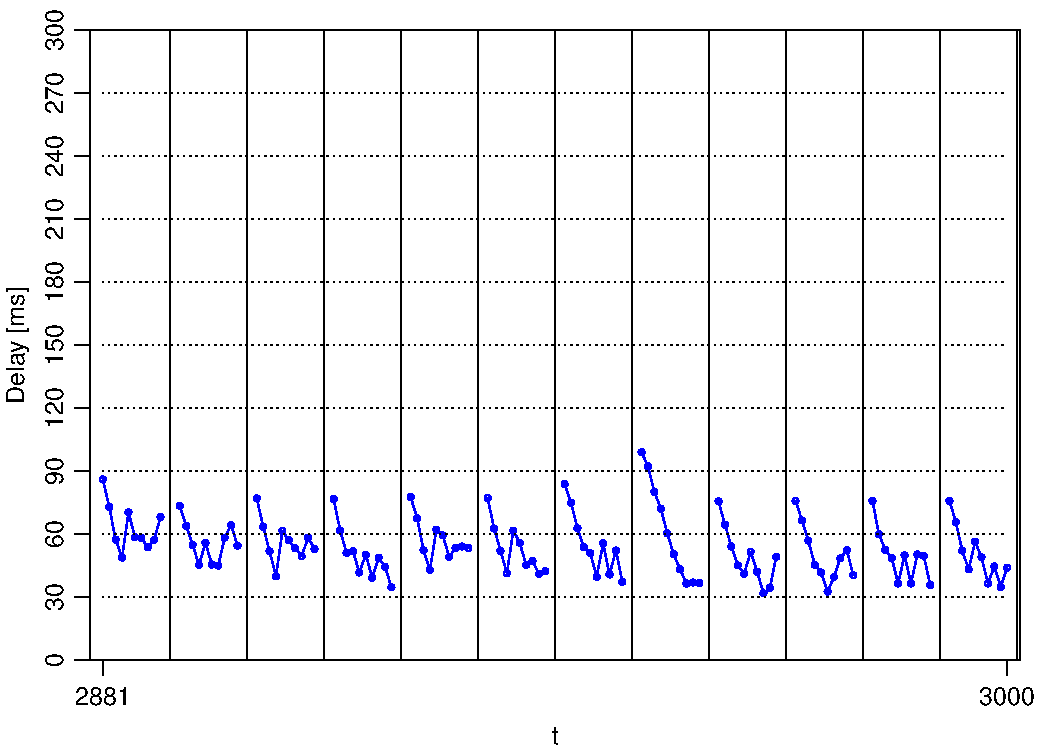
\includegraphics[width=0.33\hsize]{../2020-07-02/24-25.pdf}
}~
\subfigure[$25 \sim 26$ 分後]{
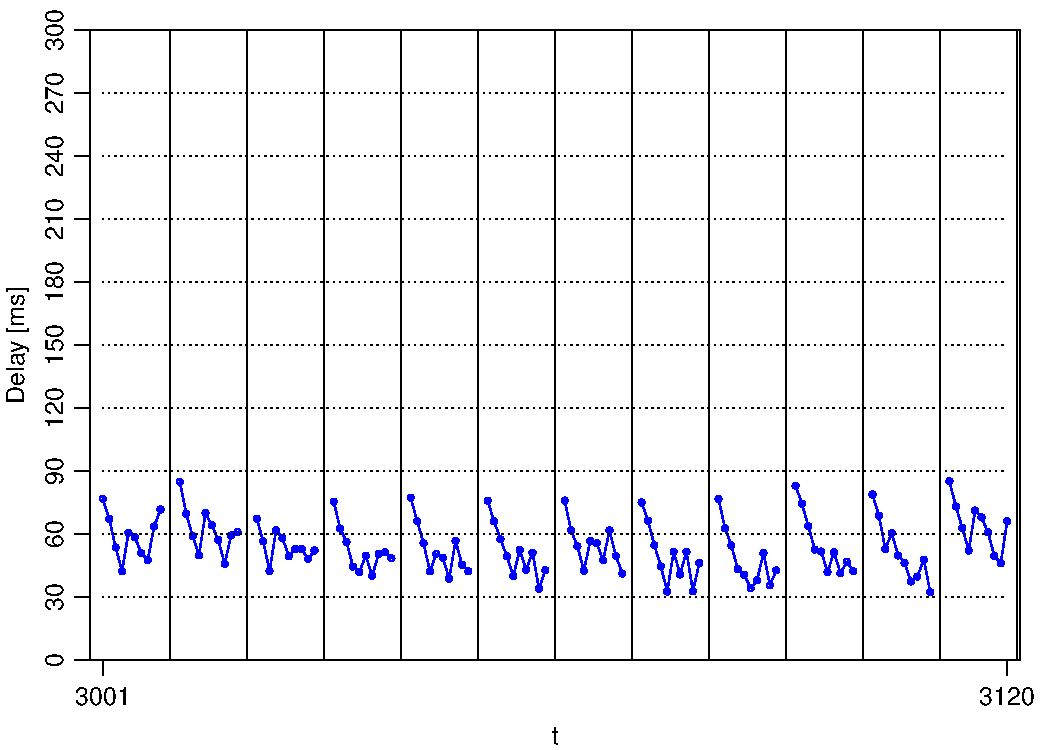
\includegraphics[width=0.33\hsize]{../2020-07-02/25-26.pdf}
}~
\subfigure[$26 \sim 27$ 分後]{
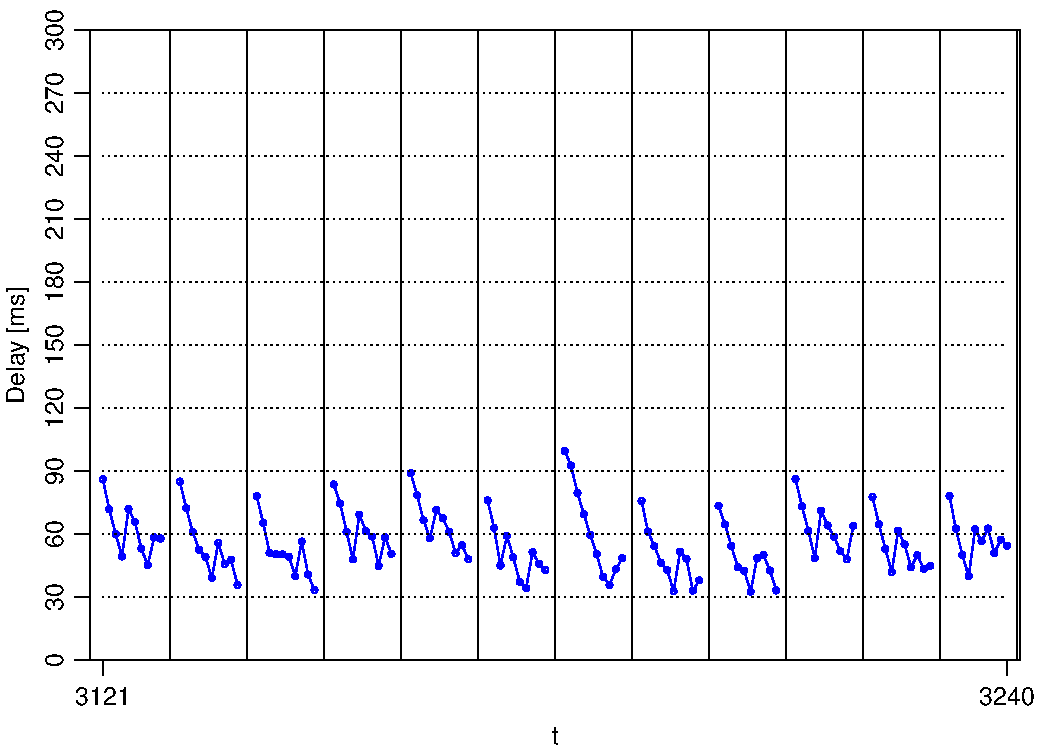
\includegraphics[width=0.33\hsize]{../2020-07-02/26-27.pdf}
}\\

\subfigure[$27 \sim 28$ 分後]{
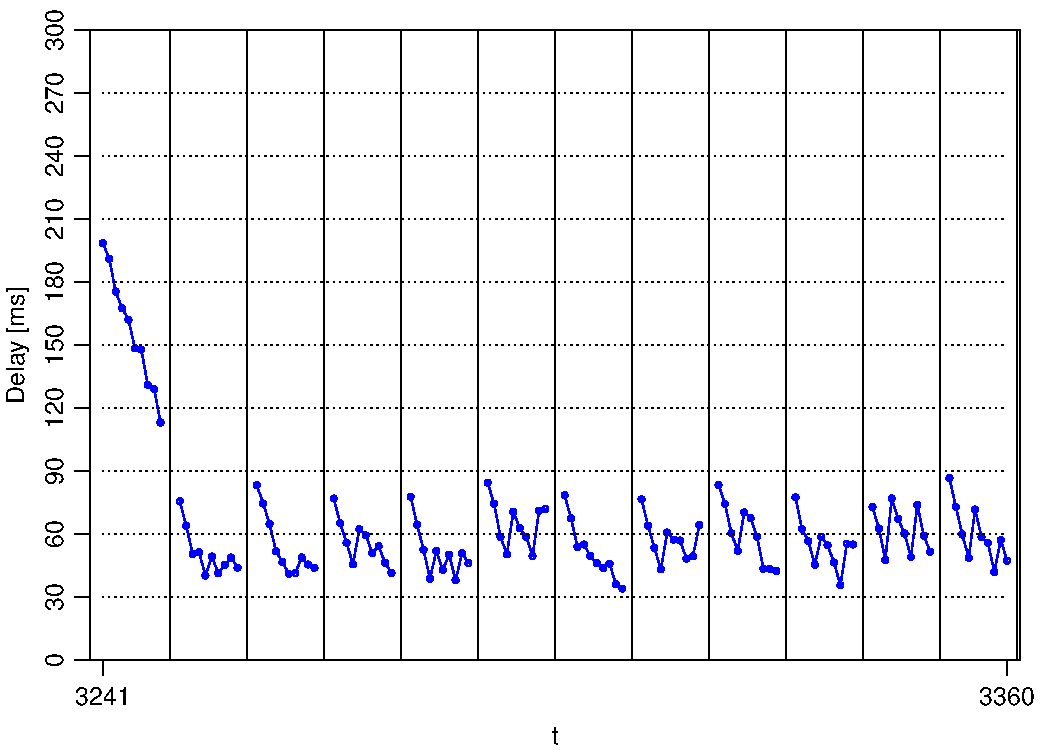
\includegraphics[width=0.33\hsize]{../2020-07-02/27-28.pdf}
}~
\subfigure[$28 \sim 29$ 分後]{
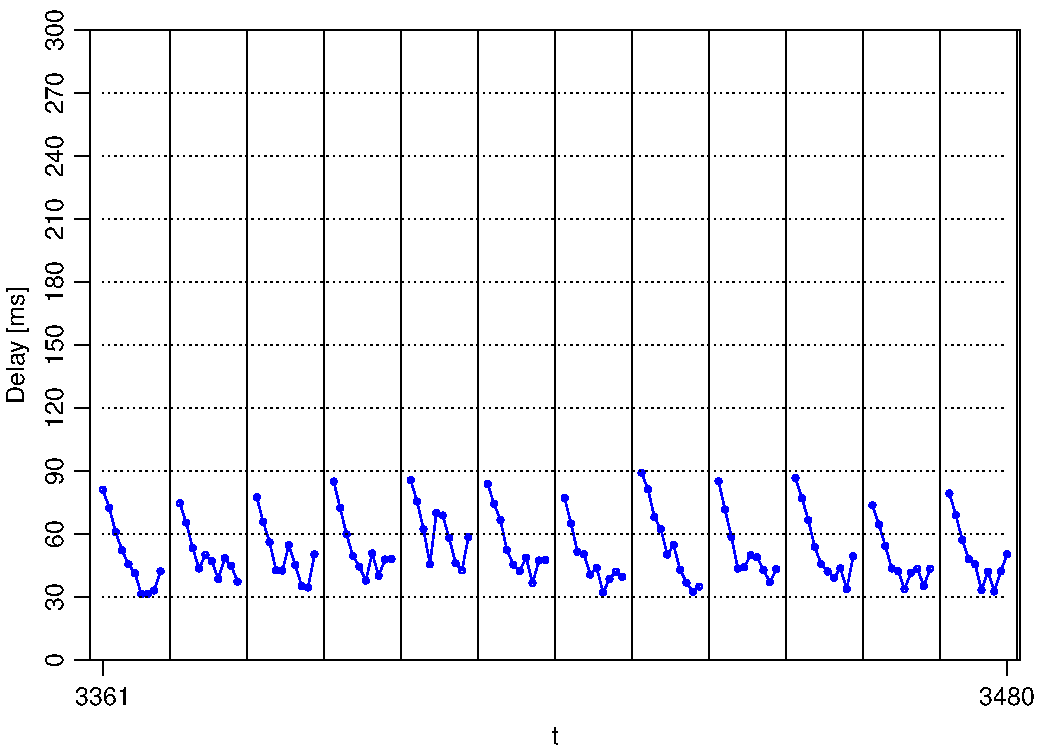
\includegraphics[width=0.33\hsize]{../2020-07-02/28-29.pdf}
}~
\subfigure[$29 \sim 30$ 分後]{
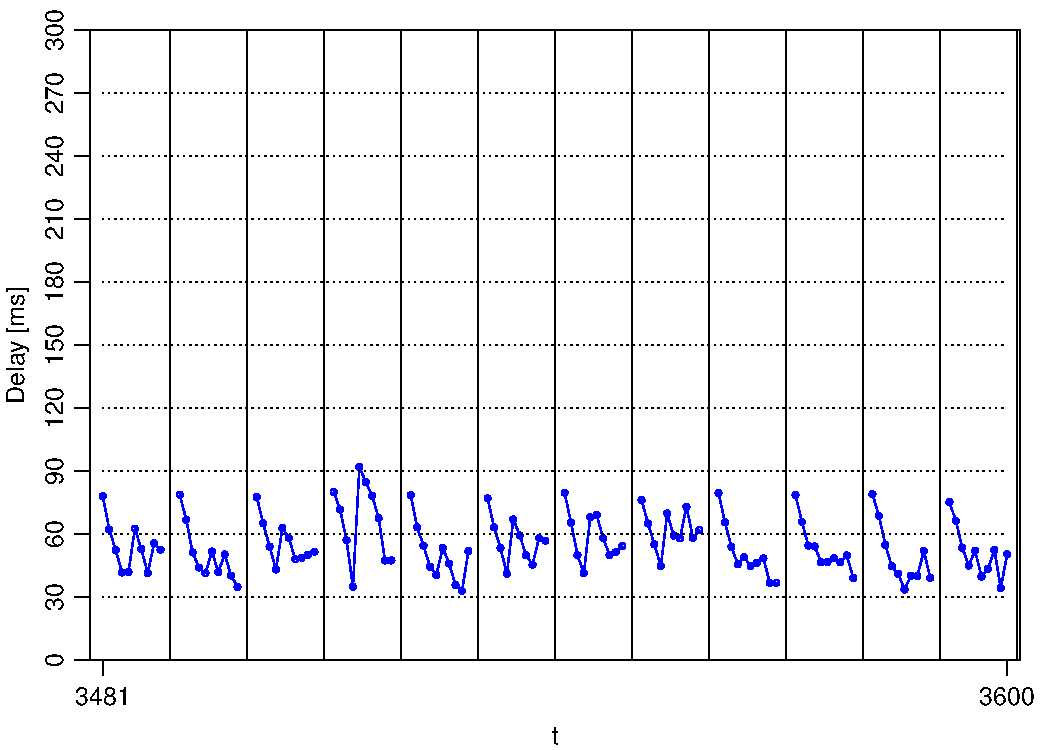
\includegraphics[width=0.33\hsize]{../2020-07-02/29-30.pdf}
}
\caption{10 ミリ秒間隔で計 10 回の ping 実行を 5 秒毎に行った計測結果(15 分後から 30 分後まで)}
\end{center}
\end{figure}

\begin{figure}[tb]
\begin{center}
\subfigure[$30 \sim 31$ 分後]{
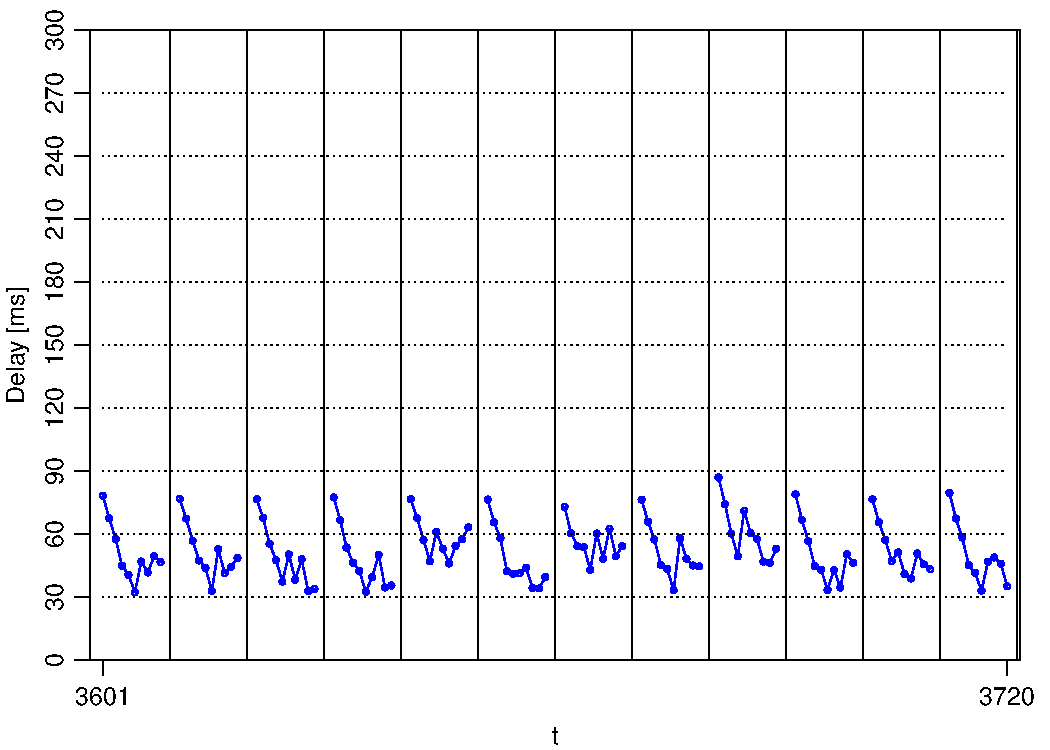
\includegraphics[width=0.33\hsize]{../2020-07-02/30-31.pdf}
}~
\subfigure[$31 \sim 32$ 分後]{
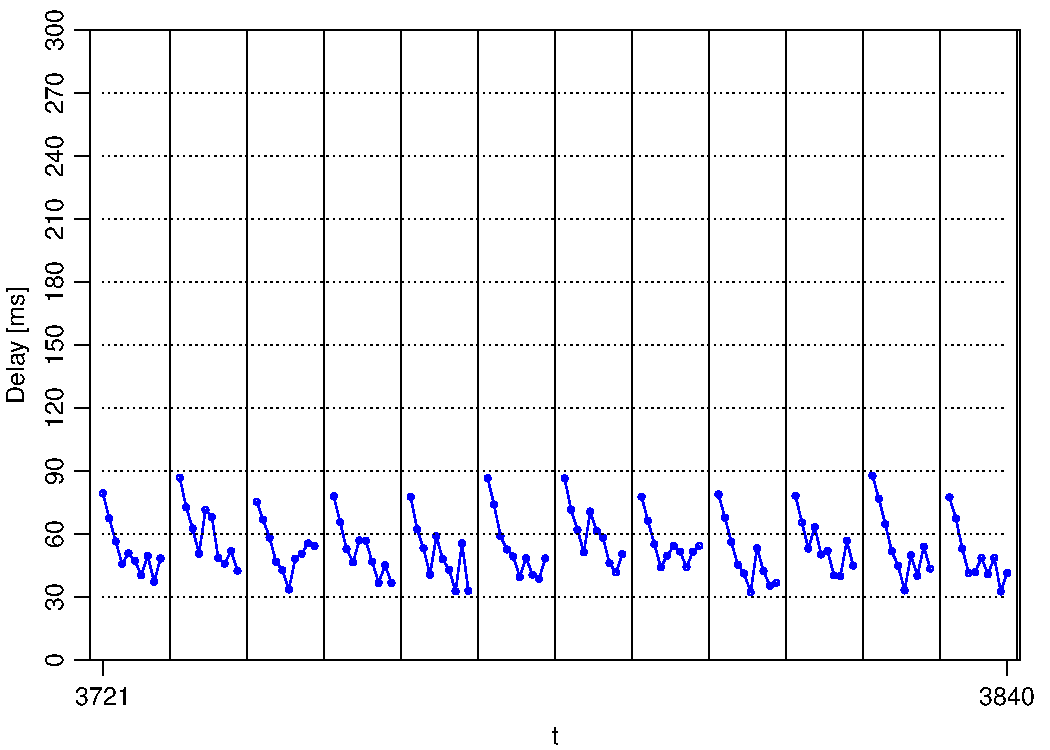
\includegraphics[width=0.33\hsize]{../2020-07-02/31-32.pdf}
}~
\subfigure[$32 \sim 33$ 分後]{
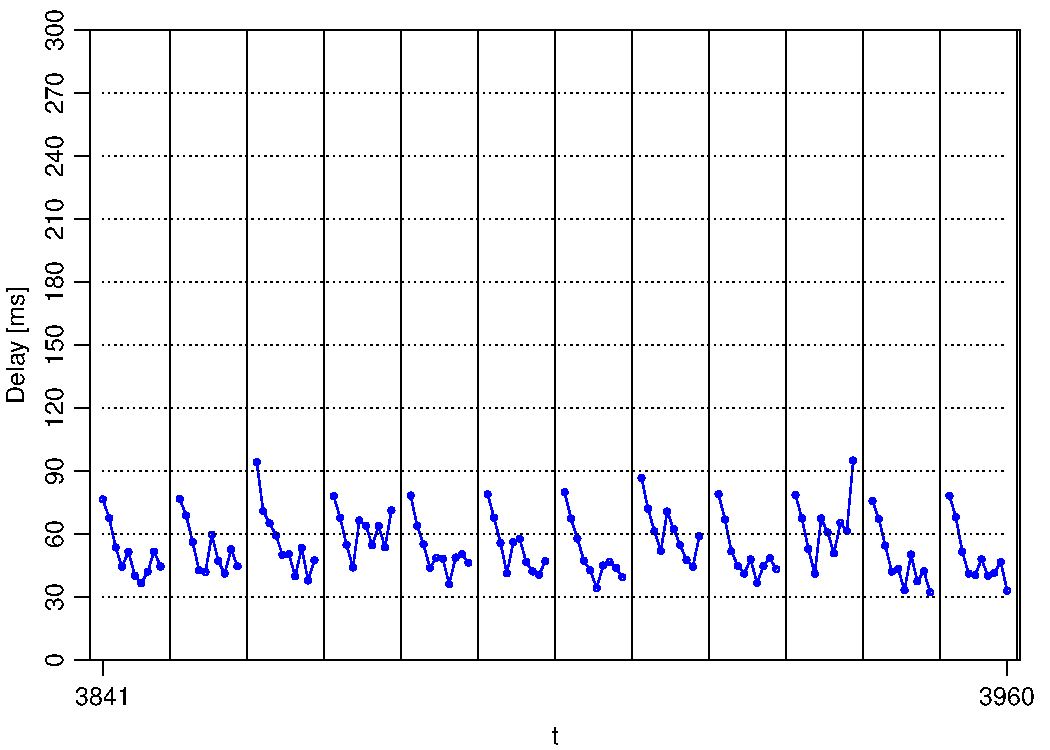
\includegraphics[width=0.33\hsize]{../2020-07-02/32-33.pdf}
}\\

\subfigure[$33 \sim 34$ 分後]{
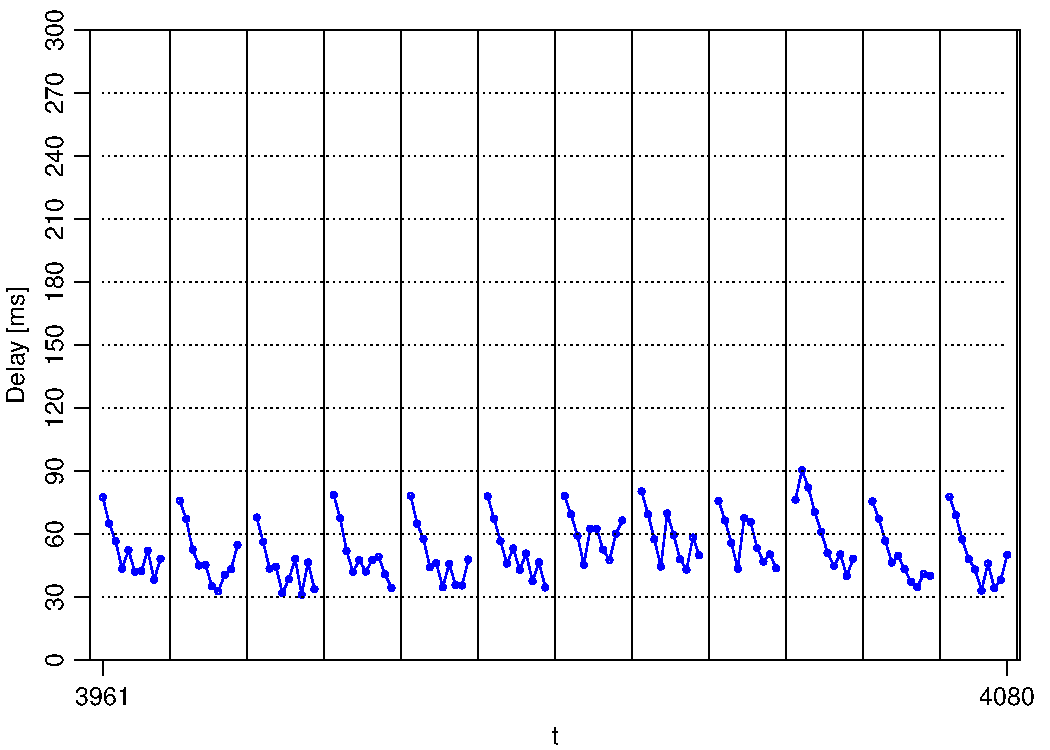
\includegraphics[width=0.33\hsize]{../2020-07-02/33-34.pdf}
}~
\subfigure[$34 \sim 35$ 分後]{
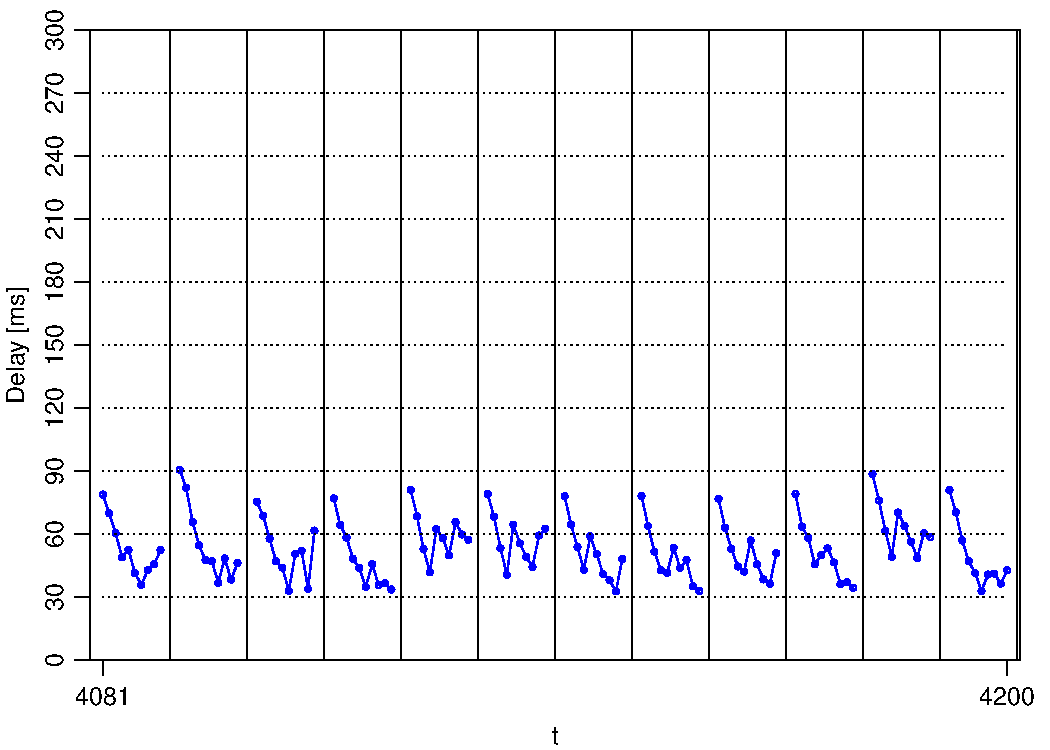
\includegraphics[width=0.33\hsize]{../2020-07-02/34-35.pdf}
}~
\subfigure[$35 \sim 36$ 分後]{
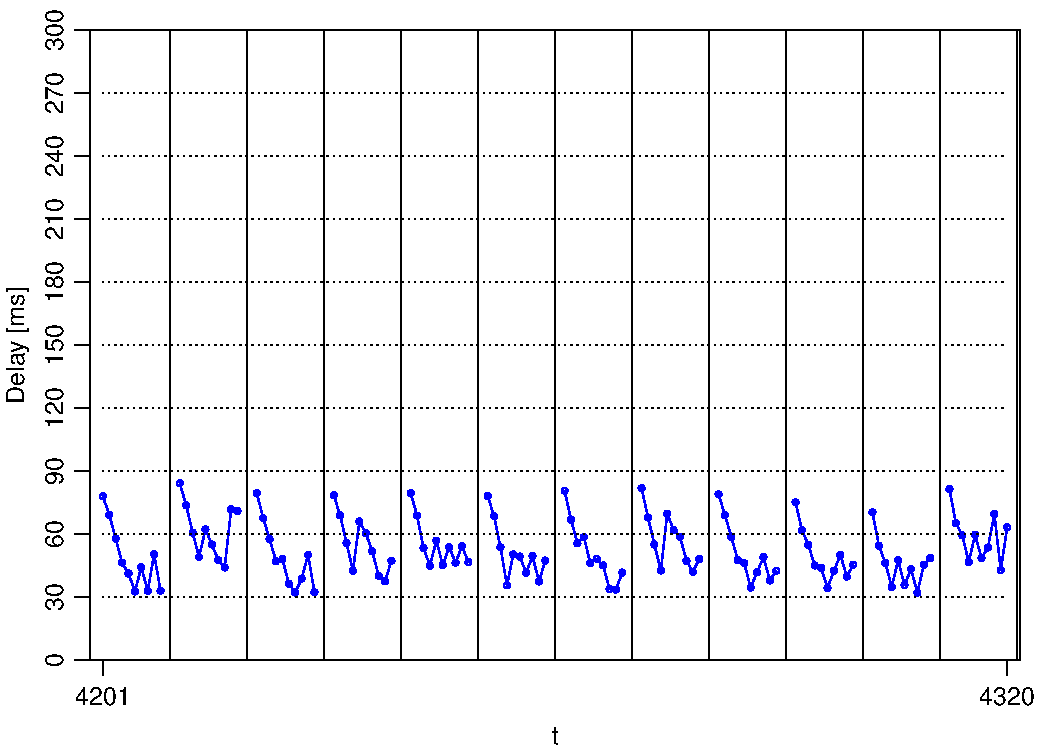
\includegraphics[width=0.33\hsize]{../2020-07-02/35-36.pdf}
}\\

\subfigure[$36 \sim 37$ 分後]{
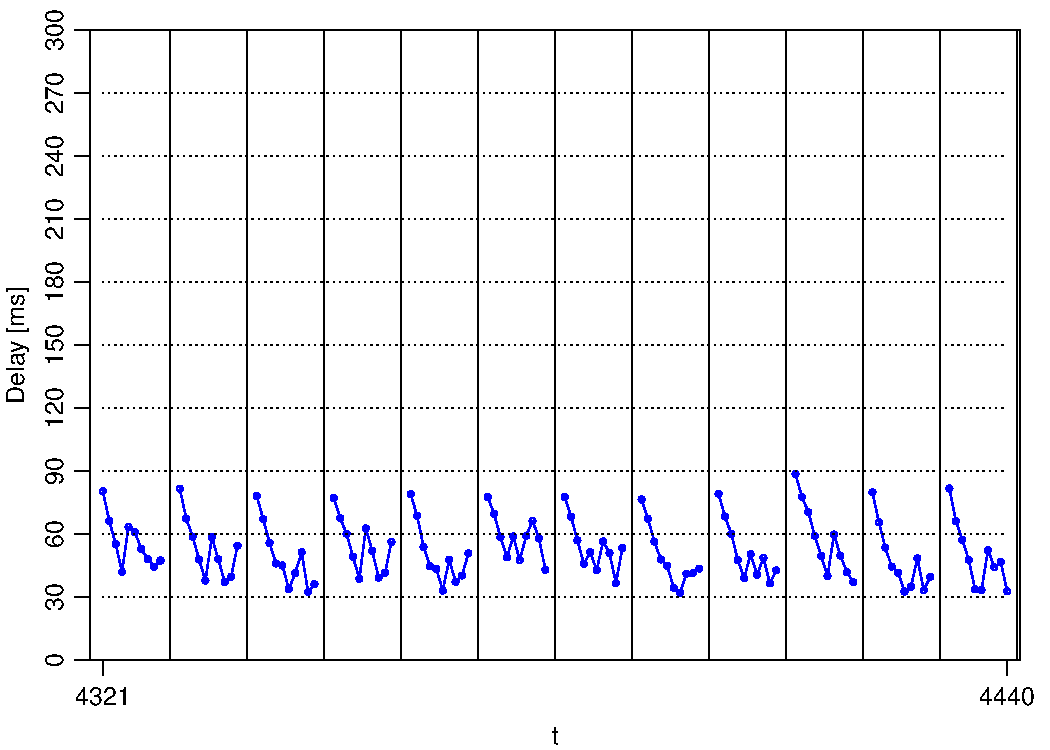
\includegraphics[width=0.33\hsize]{../2020-07-02/36-37.pdf}
}~
\subfigure[$37 \sim 38$ 分後]{
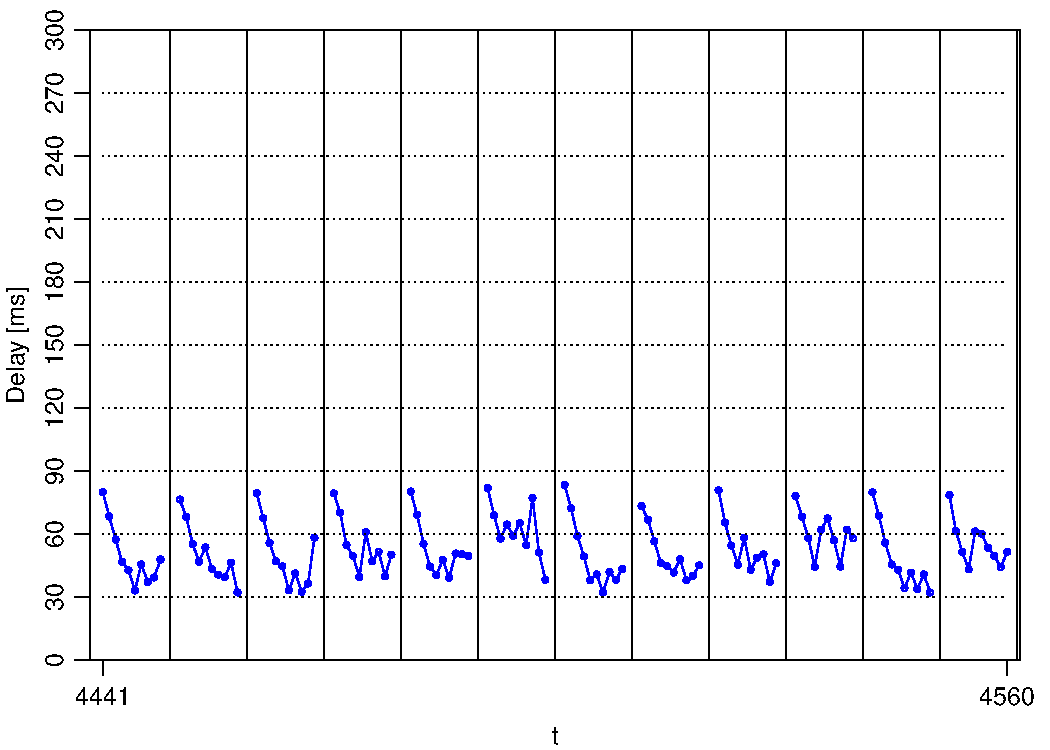
\includegraphics[width=0.33\hsize]{../2020-07-02/37-38.pdf}
}~
\subfigure[$38 \sim 39$ 分後]{
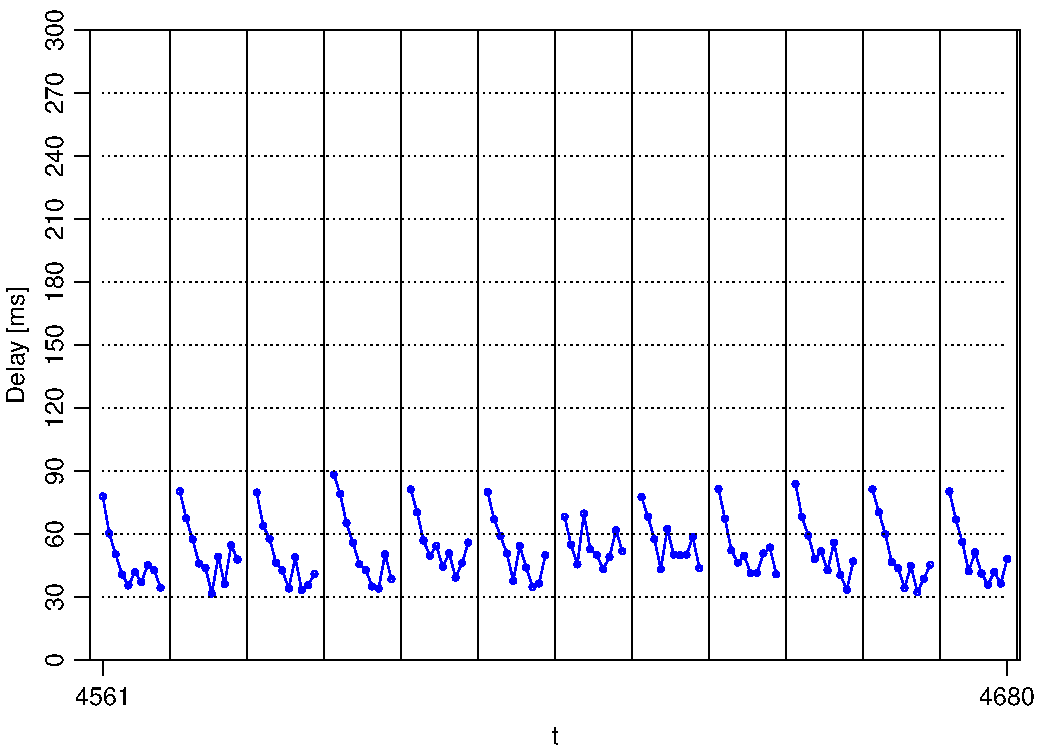
\includegraphics[width=0.33\hsize]{../2020-07-02/38-39.pdf}
}\\

\subfigure[$39 \sim 40$ 分後]{
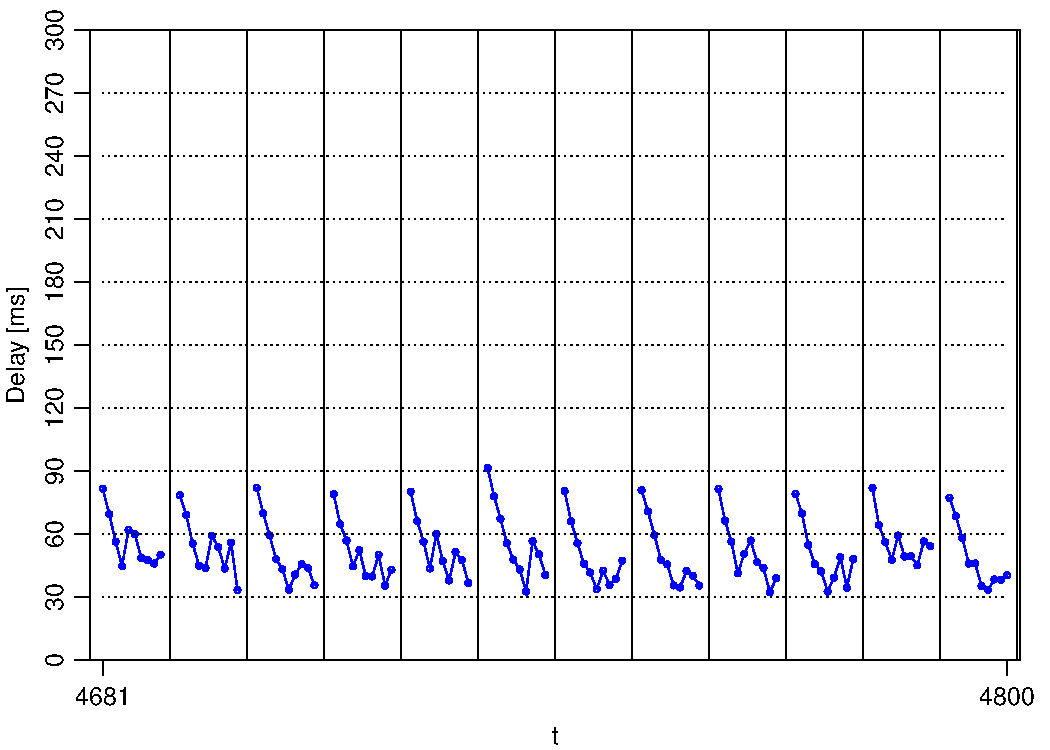
\includegraphics[width=0.33\hsize]{../2020-07-02/39-40.pdf}
}~
\subfigure[$40 \sim 41$ 分後]{
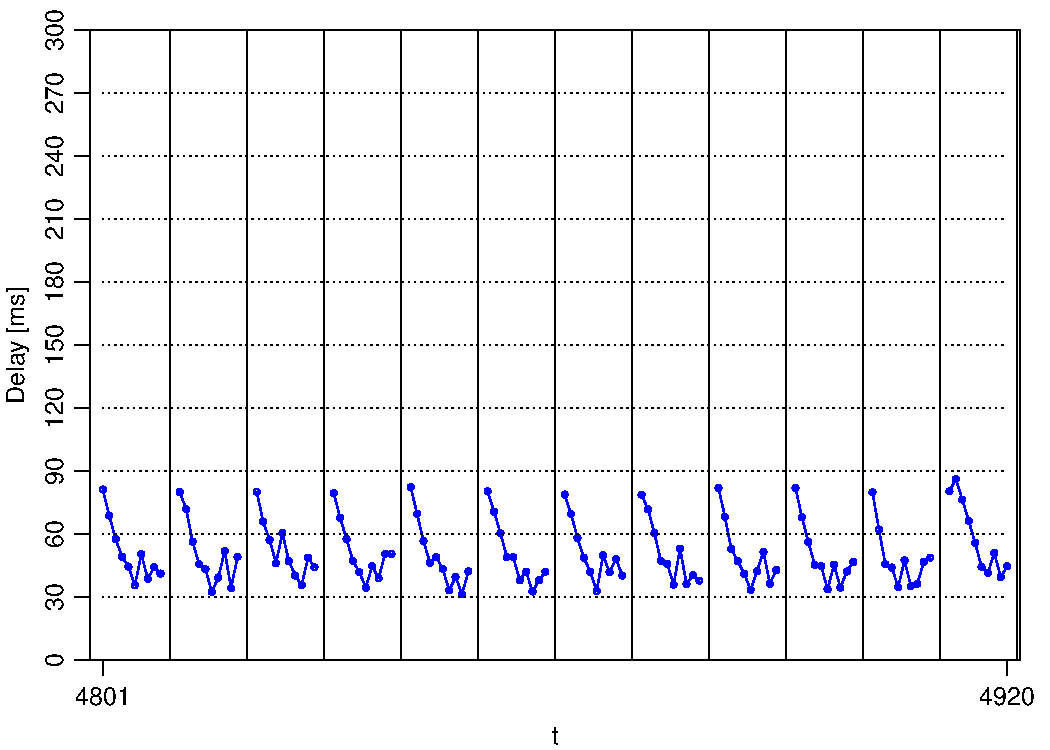
\includegraphics[width=0.33\hsize]{../2020-07-02/40-41.pdf}
}~
\subfigure[$41 \sim 42$ 分後]{
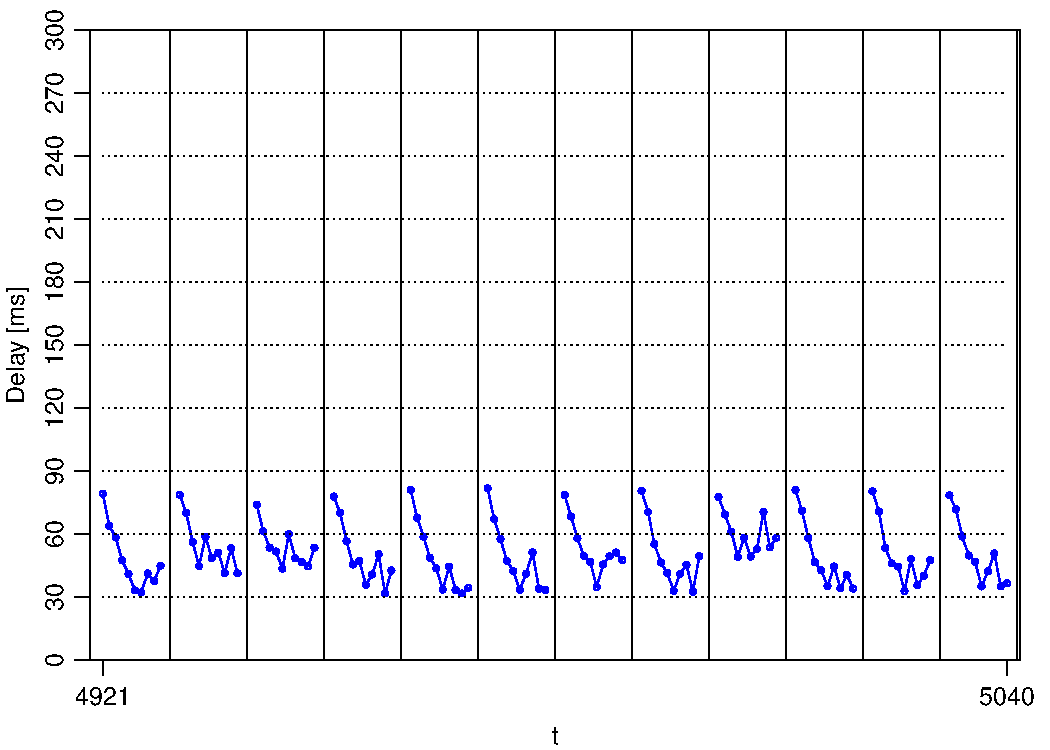
\includegraphics[width=0.33\hsize]{../2020-07-02/41-42.pdf}
}\\

\subfigure[$42 \sim 43$ 分後]{
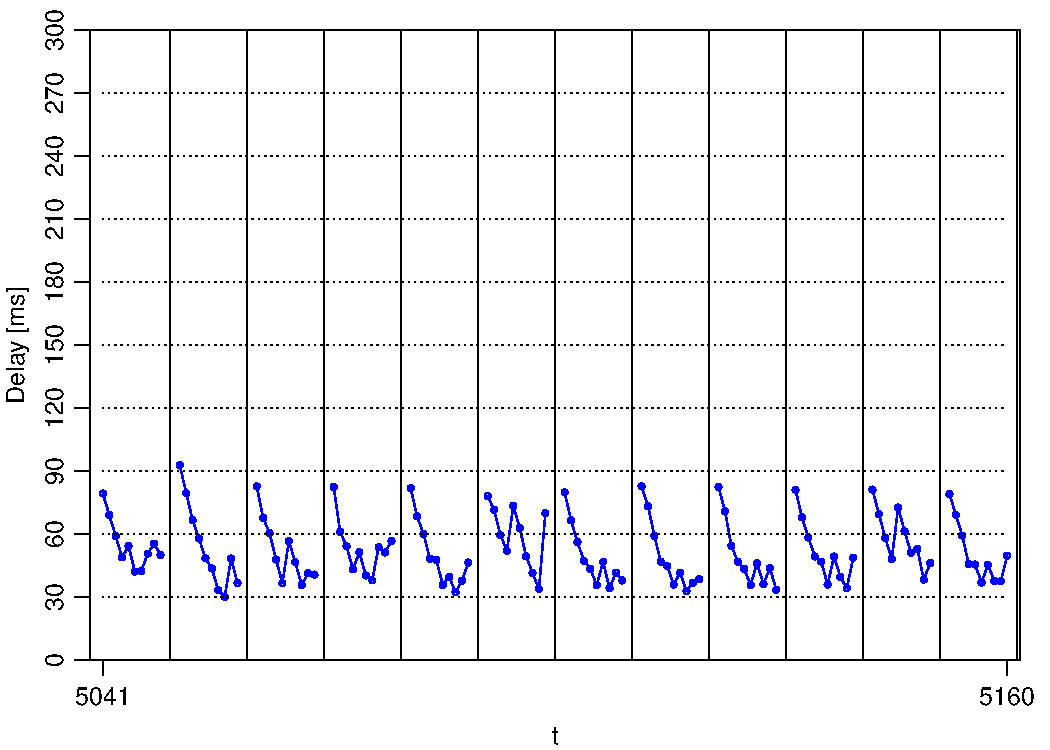
\includegraphics[width=0.33\hsize]{../2020-07-02/42-43.pdf}
}~
\subfigure[$43 \sim 44$ 分後]{
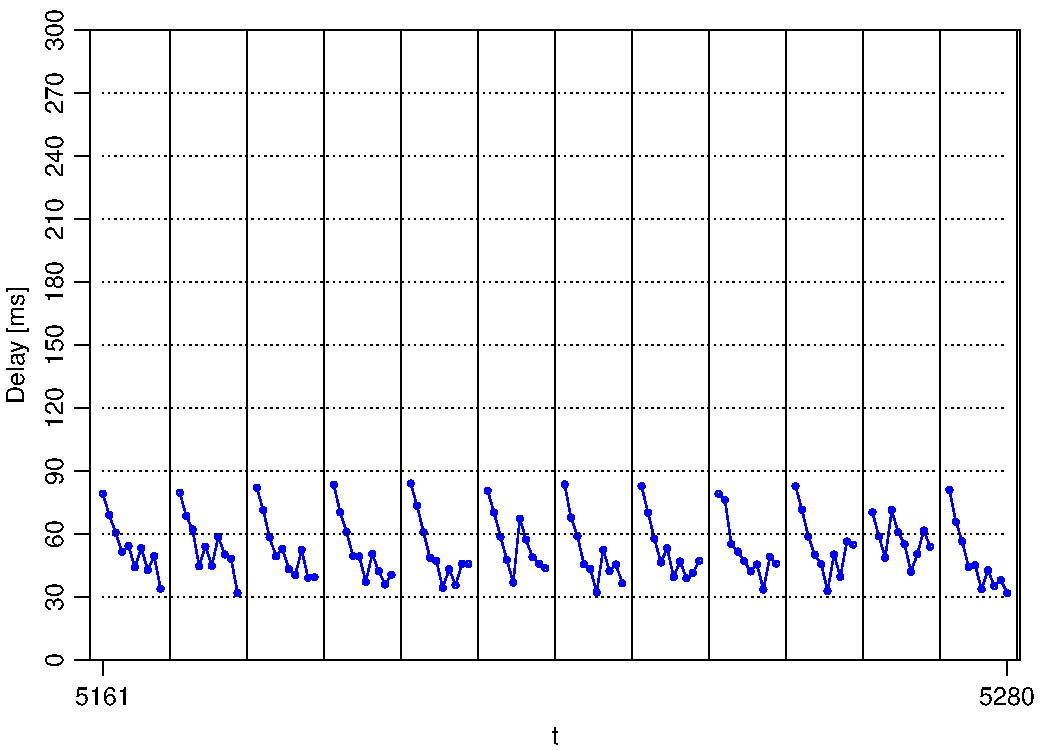
\includegraphics[width=0.33\hsize]{../2020-07-02/43-44.pdf}
}~
\subfigure[$44 \sim 45$ 分後]{
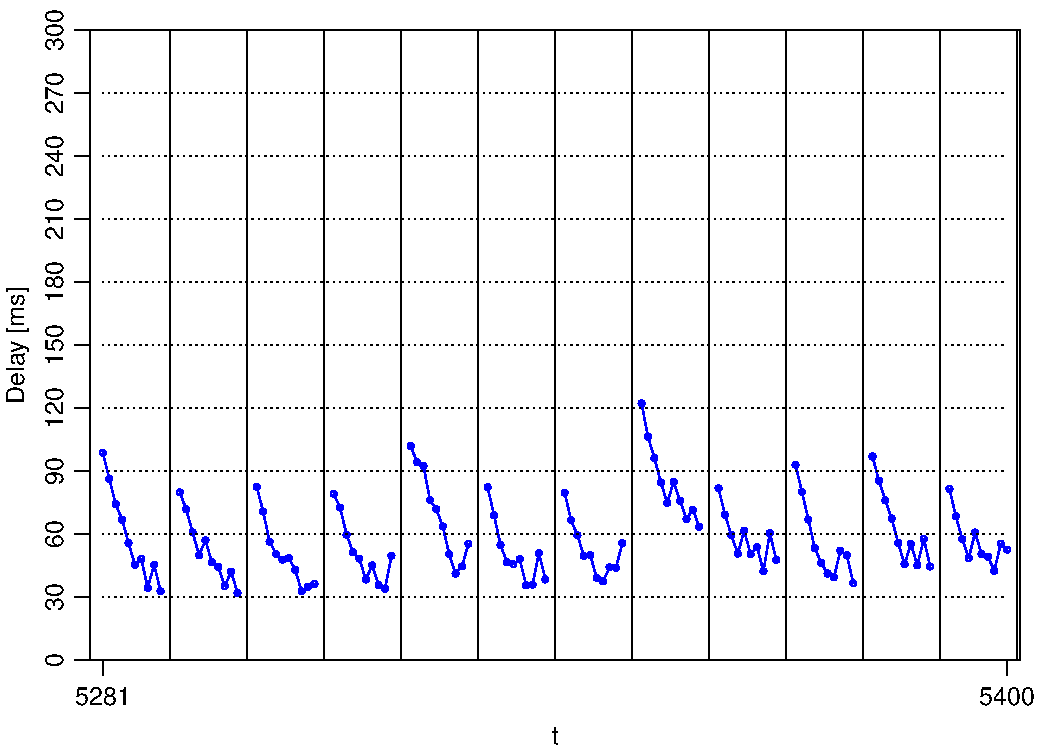
\includegraphics[width=0.33\hsize]{../2020-07-02/44-45.pdf}
}
\caption{10 ミリ秒間隔で計 10 回の ping 実行を 5 秒毎に行った計測結果(30 分後から 45 分後まで)}
\end{center}
\end{figure}

\begin{figure}[tb]
\begin{center}
\subfigure[$45 \sim 46$ 分後]{
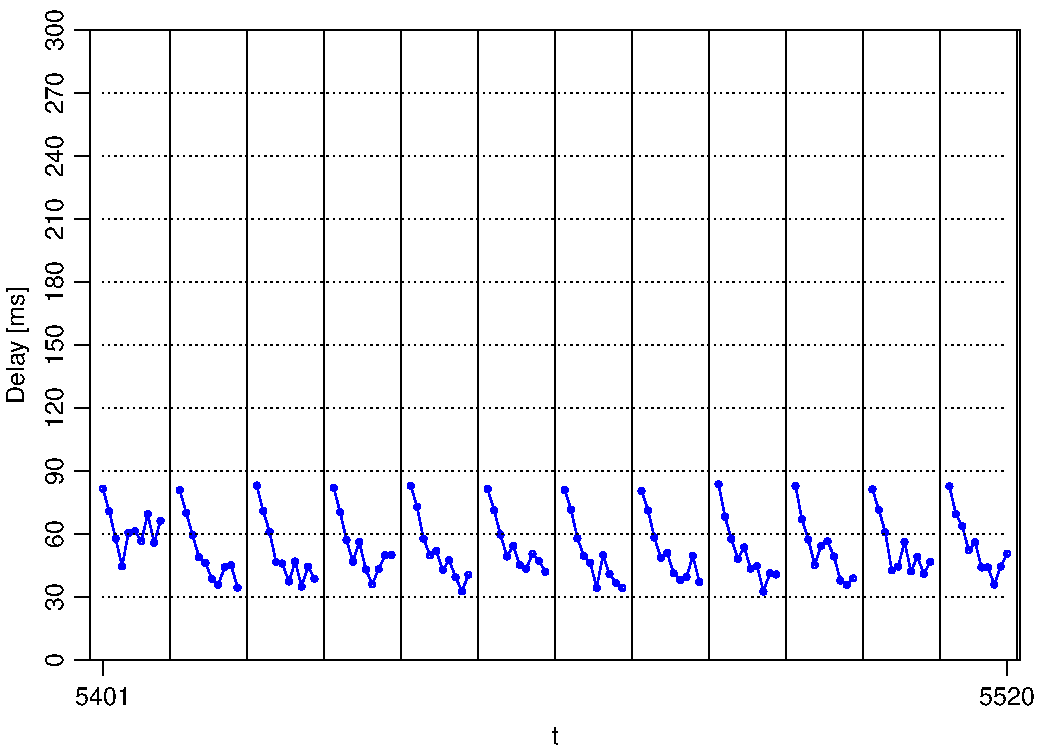
\includegraphics[width=0.33\hsize]{../2020-07-02/45-46.pdf}
}~
\subfigure[$46 \sim 47$ 分後]{
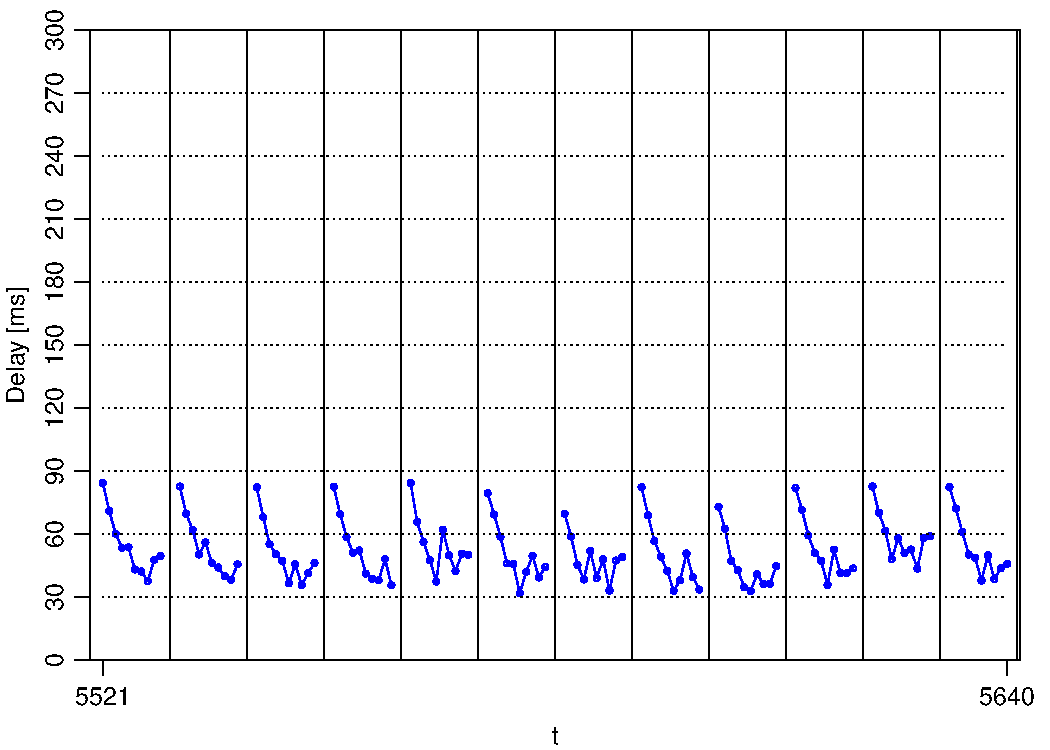
\includegraphics[width=0.33\hsize]{../2020-07-02/46-47.pdf}
}~
\subfigure[$47 \sim 48$ 分後]{
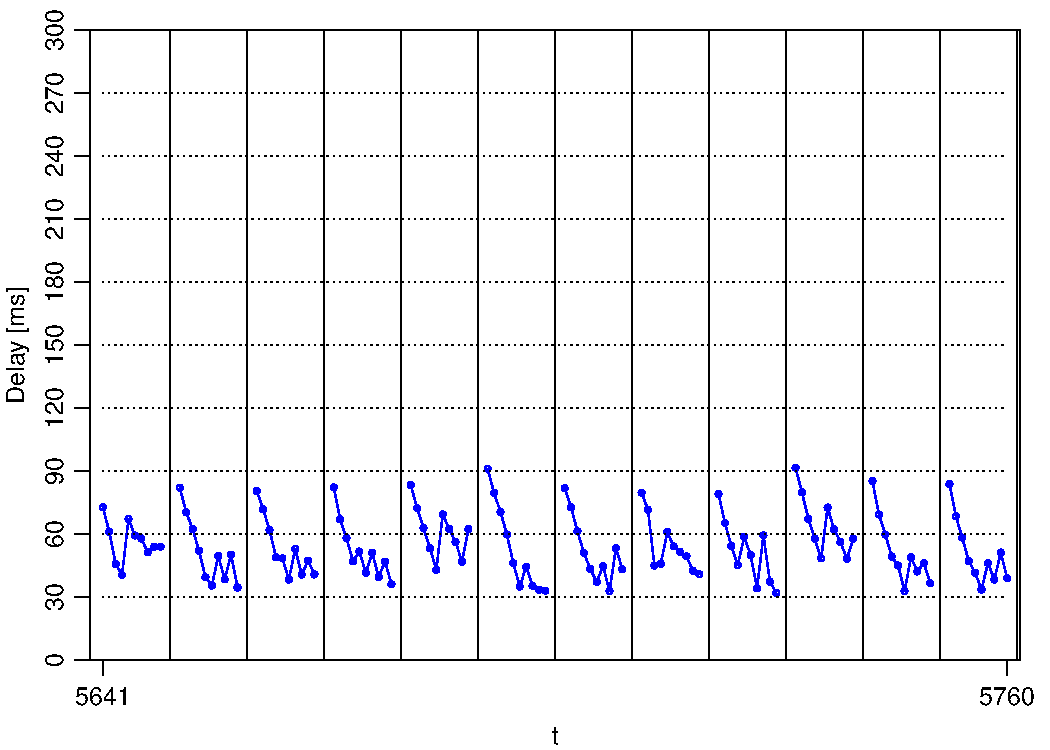
\includegraphics[width=0.33\hsize]{../2020-07-02/47-48.pdf}
}\\

\subfigure[$48 \sim 49$ 分後]{
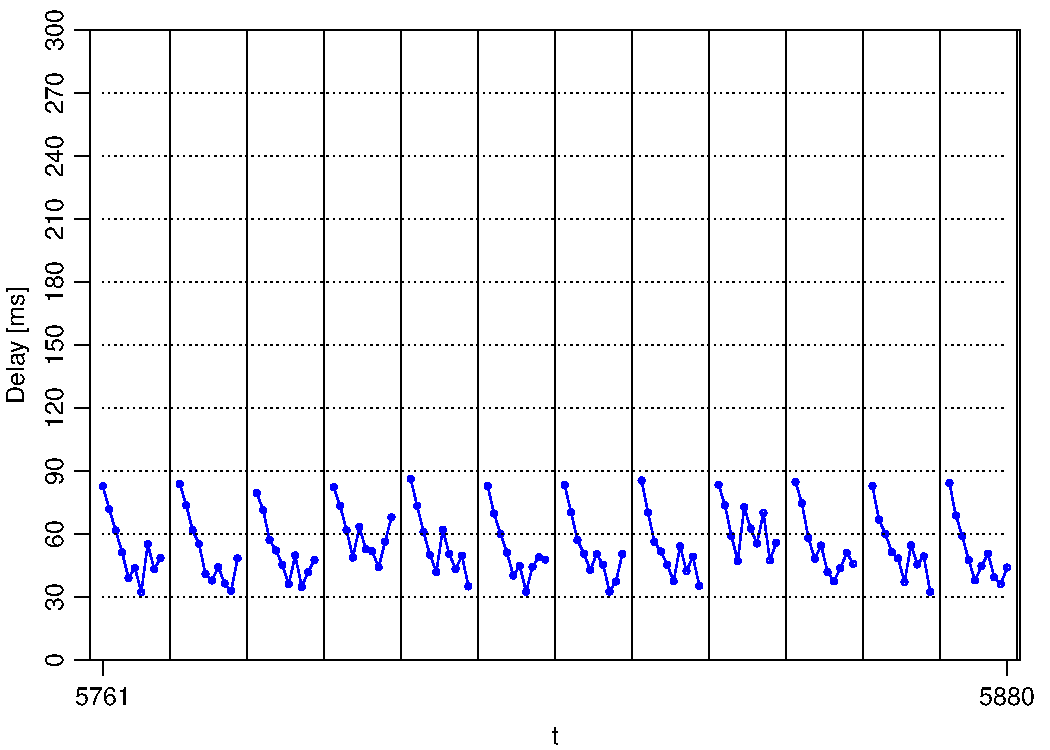
\includegraphics[width=0.33\hsize]{../2020-07-02/48-49.pdf}
}~
\subfigure[$49 \sim 50$ 分後]{
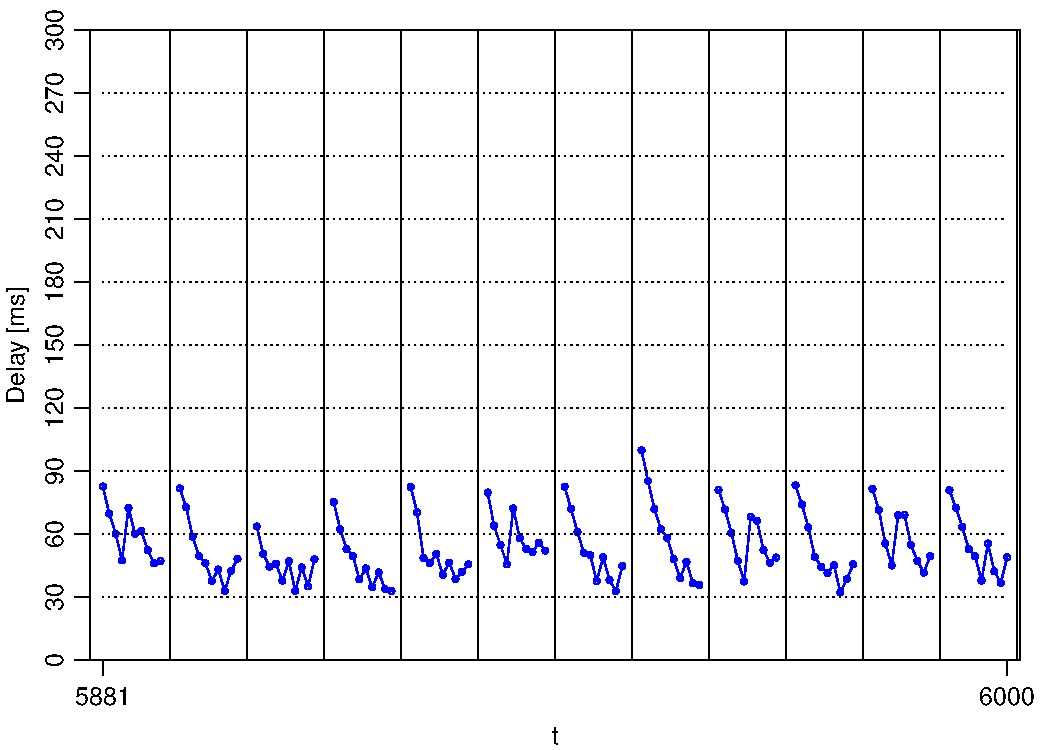
\includegraphics[width=0.33\hsize]{../2020-07-02/49-50.pdf}
}~
\subfigure[$50 \sim 51$ 分後]{
\includegraphics[width=0.33\hsize]{../2020-07-02/50-51.pdf}
}\\

\subfigure[$51 \sim 52$ 分後]{
\includegraphics[width=0.33\hsize]{../2020-07-02/51-52.pdf}
}~
\subfigure[$52 \sim 53$ 分後]{
\includegraphics[width=0.33\hsize]{../2020-07-02/52-53.pdf}
}~
\subfigure[$53 \sim 54$ 分後]{
\includegraphics[width=0.33\hsize]{../2020-07-02/53-54.pdf}
}\\

\subfigure[$54 \sim 55$ 分後]{
\includegraphics[width=0.33\hsize]{../2020-07-02/54-55.pdf}
}~
\subfigure[$55 \sim 56$ 分後]{
\includegraphics[width=0.33\hsize]{../2020-07-02/55-56.pdf}
}~
\subfigure[$56 \sim 57$ 分後]{
\includegraphics[width=0.33\hsize]{../2020-07-02/56-57.pdf}
}\\

\subfigure[$57 \sim 58$ 分後]{
\includegraphics[width=0.33\hsize]{../2020-07-02/57-58.pdf}
}~
\subfigure[$58 \sim 59$ 分後]{
\includegraphics[width=0.33\hsize]{../2020-07-02/58-59.pdf}
}~
\subfigure[$59 \sim 60$ 分後]{
\includegraphics[width=0.33\hsize]{../2020-07-02/59-60.pdf}
}
\caption{10 ミリ秒間隔で計 10 回の ping 実行を 5 秒毎に行った計測結果(45 分後から 60 分後まで)}
\label{data1-2}
\end{center}
\end{figure}

図より,組ごとに右下がりの傾向が見られ,応答遅延時間は最小応答遅延時間付近まで小さくなることが分かった.これは,後に送信される ping パケットが先に送られるパケットの影響でバッファ待ちすることなくなるからだと思われる.バッファ待ちの要因の一つとしてモバイルコアネットワークのベアラの張り直しが考えられる.この張り直しは,前の実験機器での計測において 12 秒程度の通信の途絶により発生し,5 秒では発生しないことが確認されている.SIM や OS は異なるものの,今の実験機器においても 5 秒ではベアラの張り直しは発生しないと考えた.しかしながら,図では通信間隔が最大でも 5 秒以下であるにも関わらず,10 ミリ秒間隔の最初の計測での応答遅延が大きくなっていた.したがって,今回の実験機器では,ベアラの張り直しが 5 秒程度の通信の途絶であっても発生する,もしくは,他の要因によりバッファ待ちが発生していることが考えられる.ただ,5 秒は感覚的に短くそこまで頻繁にベアラを張り直しているとは想像できないため,後者の方が可能性が高いのではないかと推測している.

\section{5 秒間隔での継続的な ping 応答遅延計測}
5 秒間隔での ping による応答遅延を一日を通じて行った.横軸に時刻をとった応答遅延の結果を図 \ref{data2} に示す.また,この計測は 7 月 1 日 15 時から 7 月 2 日 15 時までのものであり,縦の赤色点線は LTE 接続が切断された時点を表す.
\begin{figure}[tb]
\centering
\includegraphics[width=0.8\hsize]{plot5s.pdf}
\caption{ 7 月 1 日 15 時から 7 月 2 日 15 時まで(5 秒間隔)}
\label{data2}
\end{figure}
この図においても,部分的に右上がりな箇所が見て取れた.原因は現時点ではわかっていないが,5 秒という短い実行間隔であっても確認できるようだ.

\section{15 秒間隔での継続的な ping 応答遅延計測}
15 秒間隔での ping による応答遅延を一日を通じて行った.現時点では,6 月 23 日(火)から 7 月 6 日(月)までの計測結果が得られている.その結果を図 \ref{data3-1} から図 \ref{data3-2} に示す.横軸には時刻を取っており,縦軸には ping 応答遅延 [ms] を取っている.また,縦の赤色点線は LTE 接続が切断された時点を表す.
\begin{figure}[tb]
\begin{center}
\subfigure[6 月 23 日(火)]{
\includegraphics[width=0.5\hsize]{plot-6-23.pdf}
}~
\subfigure[6 月 24 日(水)]{
\includegraphics[width=0.5\hsize]{plot-6-24.pdf}
}\\
\subfigure[6 月 25 日(木)]{
\includegraphics[width=0.5\hsize]{plot-6-25.pdf}
}~
\subfigure[6 月 26 日(金)]{
\includegraphics[width=0.5\hsize]{plot-6-26.pdf}
}\\
\subfigure[6 月 27 日(土)]{
\includegraphics[width=0.5\hsize]{plot-6-27.pdf}
}~
\subfigure[6 月 28 日(日)]{
\includegraphics[width=0.5\hsize]{plot-6-28.pdf}
}
\caption{一日を通じた計測(15 秒間隔) 6 月 23 日(火)から 6 月 28 日(日)まで}
\label{data3-1}
\end{center}
\end{figure}
\begin{figure}[tb]
\begin{center}
\subfigure[6 月 29 日(月)]{
\includegraphics[width=0.5\hsize]{plot-6-29.pdf}
}~
\subfigure[6 月 30 日(火)]{
\includegraphics[width=0.5\hsize]{plot-6-30.pdf}
}\\
\subfigure[7 月 1 日(水)]{
\includegraphics[width=0.5\hsize]{plot-7-1.pdf}
}~
\subfigure[7 月 2 日(木)]{
\includegraphics[width=0.5\hsize]{plot-7-2.pdf}
}\\
\subfigure[7 月 3 日(金)]{
\includegraphics[width=0.5\hsize]{plot-7-3.pdf}
}~
\subfigure[7 月 4 日(土)]{
\includegraphics[width=0.5\hsize]{plot-7-4.pdf}
}
\caption{一日を通じた計測(15 秒間隔) 6 月 29 日(月)から 7 月 4 日(土)まで}
\label{data3}
\end{center}
\end{figure}
\begin{figure}[tb]
\begin{center}
\subfigure[7 月 5 日(日)]{
\includegraphics[width=0.5\hsize]{plot-7-5.pdf}
}~
\subfigure[7 月 6 日(月)]{
\includegraphics[width=0.5\hsize]{plot-7-6.pdf}
}
\caption{一日を通じた計測(15 秒間隔)7 月 5 日(日)と 7 月 6 日(月)}
\label{data3-2}
\end{center}
\end{figure}
この結果から新たに,図 \ref{data3-1}(b) から図 \ref{data3-1}(c) までの 6 月 24 日(水)から6 月 25 日(木)にかけて応答遅延のベースラインは大きく変わらないものの大きな応答遅延の発生頻度が極端に高くなる期間や,図 \ref{data3}(a) の 6 月 29 日(月)のように 900 ms を超えるかなり大きな応答遅延が発生する箇所が確認された.
また,いずれの図においても部分的な右上がりの傾向が見られる.

なお,応答遅延の大きさやばらつきに時間帯に応じた顕著な変化は見て取れなかった.

\section{LTE 接続の切断について}
何らかの要因でプロバイダ側から LTE 接続が切られることがある.
そのときの Raspberry Pi のログ情報は
\vspace{0.5cm}\\
11:25:59 : LCP terminated by peer       \#プロバイダ側からの切断\\
11:25:59 : Modem hangup         \#モデムの停止\\
11:25:59 : Connection terminated.    \#コネクションの切断\\
11:25:59 : candy-pi-lite start\_pppd.sh\\
\hspace{1cm}\#モデムの起動(SIM カードの読み込み・認証,APN の確認,IPアドレスの取得)\\
11:26:13 : candy-pi-lite: CANDY Pi Lite Board is initialized successfully!\\
\vspace{0.5cm}\\
となっており,大体 15 秒程度で再接続が完了するようだ.
この再接続によって UE と eNodeB,eNodeB と S-GW,S-GW と P-GW との間のベアラが解放されるかどうかは分からないが,Raspberry Pi に電源を入れたときと同様に,candy-pi-lite start\_pppd.sh を用いたモデムの起動と接続要求を行っていることから,復帰直後はベアラが張られた状態になっていると考えられる.よって,LTE 接続切れの直後の応答遅延が大きくなるわけではないと思われる.表 \ref{1} は 図 \ref{data3-1} から図 \ref{data3-2} において赤色点線で示される LTE 接続切れが起こった時点の時刻と直前と直後のそれぞれの計測の応答遅延時間を示したものである.
\begin{table}[tb]
\centering
\caption{LTE 接続切れの前後の応答遅延}
\label{1}
\begin{tabular}{|c|c|c|}
\hline
LTE 接続切れの時刻&直前の応答遅延 [ms] &直後の応答遅延 [ms]\\
\hline
6/23 18:14 & 88.934 & 73.963\\
\hline
6/24 5:12 & 72.752 & 74.752\\
\hline
6/24 17:39 & 67.805 & 69.993\\
\hline
6/24 18:22 & 89.047 & 96.564\\
\hline
6/24 18:58 & 73.25 & 72.536\\
\hline
6/25 7:58& 99.517 & 73.378\\
\hline
6/25 11:23 & 77.071 & 88.349\\
\hline
6/26 11:23 & 72.568 & 82.324\\
\hline
6/27 11:23 & 78.957 & 81.854\\
\hline
6/28 11:23 & 74.188 & 90.633\\
\hline
6/29 11:24 & 78.807 & 89.982\\
\hline
6/30 11:24 & 98.668 & 87.294\\
\hline
7/1 11:24  & 76.881 & 103.859\\
\hline
7/2 11:24  & 74.716 & 88.716\\
\hline
7/3 11:24  & 74.385 & 87.174\\
\hline
7/3 16:06  & 76.791 & 76.731\\
\hline
7/3 18:20  & 73.014 & 71.303\\
\hline
7/4 11:23  & 78.397 & 81.959\\
\hline
7/5 11:24  & 78.295 & 78.767\\
\hline
7/5 12:17  & 81.315 & 72.903\\
\hline
7/6 11:25  & 89.076 & 84.182\\
\hline
7/6 12:29  & 80.295 & 80.794\\
\hline
\end{tabular}
\end{table}
この表から,直後の応答遅延は図 1 (a) で見られるようなベアラ構築が必要と考えられる最初の計測で得られる 300 ms 程度と比べて十分小さく,他の多くの応答遅延が分布している 60 ms から 90 ms の範囲内であることが見て取れ,再接続後にはその直後から通常通りの応答遅延時間を取ることがわかる.
また,直前の応答遅延もこの分布帯の範囲内であり,LTE 接続がプロバイダ側から切られる兆候があるようには思えなかった.
また,6/25 以降は 11:25 ごろにこの接続切れが発生していた.
この時刻になると接続を一度切る設定が Raspberry Pi にあるのかと思えたが 6/23 などは行っていないことからそうではないようだ.
連続接続時間が 24 時間である可能性も考えたが,途中(7/3 11:24 から 7/4 11:23 までの間の 7/3 16:06 など)でLTE 接続切れが発生しても次の 11:25 ごろに 24 時間の経過を待たずに発生していることからこれも考えにくい.
よって,時刻依存であることは確かとは思うが,その設定は Raspberry Pi 側ではなくプロバイダ側が行っていると思われる.

\section{inactivity timer}
コアネットワーク内のタイマーについて調べた.なお,産業用モニタリングシステムにおける無線端末の移動は考えにくいため,ハンドオーバーなどの端末移動に伴った処理に関するタイマーは除いている.
今回私が見つけられたものは inactivity timer だけです.
このタイマーは,UE がある程度の時間通信を行わないと発生する,UE と eNodeB,eNodeB と S-GW との間のベアラの解放が行われるまでの時間を計るものである.このタイマーの値は各通信事業者が個別に設定することが可能であり,また,通信の混雑具合から動的に変更しているようだ\cite{chen2015analysis}.
ただ,このタイマーの値を計るとおよそ 120 秒程度であったという報告\cite{1}があり,私の実験設定においても大体その程度なのではないかと思われる.
\bibliography{myref}
\bibliographystyle{../sieicej}
\end{document}